\documentclass[twoside]{book}

% Packages required by doxygen
\usepackage{fixltx2e}
\usepackage{calc}
\usepackage{doxygen}
\usepackage[export]{adjustbox} % also loads graphicx
\usepackage{graphicx}
\usepackage[utf8]{inputenc}
\usepackage{makeidx}
\usepackage{multicol}
\usepackage{multirow}
\PassOptionsToPackage{warn}{textcomp}
\usepackage{textcomp}
\usepackage[nointegrals]{wasysym}
\usepackage[table]{xcolor}

% Font selection
\usepackage[T1]{fontenc}
\usepackage[scaled=.90]{helvet}
\usepackage{courier}
\usepackage{amssymb}
\usepackage{sectsty}
\renewcommand{\familydefault}{\sfdefault}
\allsectionsfont{%
  \fontseries{bc}\selectfont%
  \color{darkgray}%
}
\renewcommand{\DoxyLabelFont}{%
  \fontseries{bc}\selectfont%
  \color{darkgray}%
}
\newcommand{\+}{\discretionary{\mbox{\scriptsize$\hookleftarrow$}}{}{}}

% Page & text layout
\usepackage{geometry}
\geometry{%
  a4paper,%
  top=2.5cm,%
  bottom=2.5cm,%
  left=2.5cm,%
  right=2.5cm%
}
\tolerance=750
\hfuzz=15pt
\hbadness=750
\setlength{\emergencystretch}{15pt}
\setlength{\parindent}{0cm}
\setlength{\parskip}{3ex plus 2ex minus 2ex}
\makeatletter
\renewcommand{\paragraph}{%
  \@startsection{paragraph}{4}{0ex}{-1.0ex}{1.0ex}{%
    \normalfont\normalsize\bfseries\SS@parafont%
  }%
}
\renewcommand{\subparagraph}{%
  \@startsection{subparagraph}{5}{0ex}{-1.0ex}{1.0ex}{%
    \normalfont\normalsize\bfseries\SS@subparafont%
  }%
}
\makeatother

% Headers & footers
\usepackage{fancyhdr}
\pagestyle{fancyplain}
\fancyhead[LE]{\fancyplain{}{\bfseries\thepage}}
\fancyhead[CE]{\fancyplain{}{}}
\fancyhead[RE]{\fancyplain{}{\bfseries\leftmark}}
\fancyhead[LO]{\fancyplain{}{\bfseries\rightmark}}
\fancyhead[CO]{\fancyplain{}{}}
\fancyhead[RO]{\fancyplain{}{\bfseries\thepage}}
\fancyfoot[LE]{\fancyplain{}{}}
\fancyfoot[CE]{\fancyplain{}{}}
\fancyfoot[RE]{\fancyplain{}{\bfseries\scriptsize Generated by Doxygen }}
\fancyfoot[LO]{\fancyplain{}{\bfseries\scriptsize Generated by Doxygen }}
\fancyfoot[CO]{\fancyplain{}{}}
\fancyfoot[RO]{\fancyplain{}{}}
\renewcommand{\footrulewidth}{0.4pt}
\renewcommand{\chaptermark}[1]{%
  \markboth{#1}{}%
}
\renewcommand{\sectionmark}[1]{%
  \markright{\thesection\ #1}%
}

% Indices & bibliography
\usepackage{natbib}
\usepackage[titles]{tocloft}
\setcounter{tocdepth}{3}
\setcounter{secnumdepth}{5}
\makeindex

% Hyperlinks (required, but should be loaded last)
\usepackage{ifpdf}
\ifpdf
  \usepackage[pdftex,pagebackref=true]{hyperref}
\else
  \usepackage[ps2pdf,pagebackref=true]{hyperref}
\fi
\hypersetup{%
  colorlinks=true,%
  linkcolor=blue,%
  citecolor=blue,%
  unicode%
}

% Custom commands
\newcommand{\clearemptydoublepage}{%
  \newpage{\pagestyle{empty}\cleardoublepage}%
}

\usepackage{caption}
\captionsetup{labelsep=space,justification=centering,font={bf},singlelinecheck=off,skip=4pt,position=top}

%===== C O N T E N T S =====

\begin{document}

% Titlepage & ToC
\hypersetup{pageanchor=false,
             bookmarksnumbered=true,
             pdfencoding=unicode
            }
\pagenumbering{alph}
\begin{titlepage}
\vspace*{7cm}
\begin{center}%
{\Large My Project }\\
\vspace*{1cm}
{\large Generated by Doxygen 1.8.13}\\
\end{center}
\end{titlepage}
\clearemptydoublepage
\pagenumbering{roman}
\tableofcontents
\clearemptydoublepage
\pagenumbering{arabic}
\hypersetup{pageanchor=true}

%--- Begin generated contents ---
\chapter{Hierarchical Index}
\section{Class Hierarchy}
This inheritance list is sorted roughly, but not completely, alphabetically\+:\begin{DoxyCompactList}
\item \contentsline{section}{translation\+Visualization.\+Data\+Reader}{\pageref{classtranslation_visualization_1_1_data_reader}}{}
\item \contentsline{section}{translation\+Visualization.\+Item}{\pageref{classtranslation_visualization_1_1_item}}{}
\item \contentsline{section}{translation\+Visualization.\+Lemma\+Process}{\pageref{classtranslation_visualization_1_1_lemma_process}}{}
\item \contentsline{section}{translation\+Visualization.\+Main\+Method}{\pageref{classtranslation_visualization_1_1_main_method}}{}
\item \contentsline{section}{translation\+Visualization.\+T\+F\+I\+D\+F\+Calculator}{\pageref{classtranslation_visualization_1_1_t_f_i_d_f_calculator}}{}
\item \contentsline{section}{translation\+Visualization.\+Translation\+Visualization}{\pageref{classtranslation_visualization_1_1_translation_visualization}}{}
\item \contentsline{section}{translation\+Visualization.\+Version}{\pageref{classtranslation_visualization_1_1_version}}{}
\item J\+Panel\begin{DoxyCompactList}
\item \contentsline{section}{translation\+Visualization.\+Rectangle}{\pageref{classtranslation_visualization_1_1_rectangle}}{}
\end{DoxyCompactList}
\end{DoxyCompactList}

\chapter{Class Index}
\section{Class List}
Here are the classes, structs, unions and interfaces with brief descriptions\+:\begin{DoxyCompactList}
\item\contentsline{section}{\hyperlink{classtranslation_visualizaton_g_u_i_1_1_color_legend_panel}{translation\+Visualizaton\+G\+U\+I.\+Color\+Legend\+Panel} }{\pageref{classtranslation_visualizaton_g_u_i_1_1_color_legend_panel}}{}
\item\contentsline{section}{\hyperlink{classtranslation_visualizaton_g_u_i_1_1_concordance_panel}{translation\+Visualizaton\+G\+U\+I.\+Concordance\+Panel} }{\pageref{classtranslation_visualizaton_g_u_i_1_1_concordance_panel}}{}
\item\contentsline{section}{\hyperlink{classtranslation_visualizaton_g_u_i_1_1_version_chosen_panel}{translation\+Visualizaton\+G\+U\+I.\+Version\+Chosen\+Panel} }{\pageref{classtranslation_visualizaton_g_u_i_1_1_version_chosen_panel}}{}
\end{DoxyCompactList}

\chapter{Class Documentation}
\hypertarget{classtranslation_visualization_1_1_data_reader}{}\section{translation\+Visualization.\+Data\+Reader Class Reference}
\label{classtranslation_visualization_1_1_data_reader}\index{translation\+Visualization.\+Data\+Reader@{translation\+Visualization.\+Data\+Reader}}
\subsection*{Public Member Functions}
\begin{DoxyCompactItemize}
\item 
List$<$ Hashtable$<$ String, Integer $>$ $>$ \hyperlink{classtranslation_visualization_1_1_data_reader_a9f7d0eb449890ad6fcf871f79f7a614c}{get\+M\+\_\+token\+Lists} ()
\item 
void \hyperlink{classtranslation_visualization_1_1_data_reader_a6ae3b7c60cbbad3269bc35c03e25b65d}{set\+M\+\_\+\+One\+Token\+List} (List$<$ String $>$ m\+\_\+\+One\+Token\+List)
\item 
List$<$ String $>$ \hyperlink{classtranslation_visualization_1_1_data_reader_a4f289a631f261a4c1f2cc1ba67fa755a}{get\+M\+\_\+\+One\+Token\+List} ()
\item 
\mbox{\Hypertarget{classtranslation_visualization_1_1_data_reader_afbf6285cc3386ca40da206de79639610}\label{classtranslation_visualization_1_1_data_reader_afbf6285cc3386ca40da206de79639610}} 
List$<$ Map.\+Entry$<$ String, Integer $>$ $>$ {\bfseries get\+M\+\_\+\+Frequency\+Index} ()
\item 
\mbox{\Hypertarget{classtranslation_visualization_1_1_data_reader_ab55bcf952d5471424844eb0821269247}\label{classtranslation_visualization_1_1_data_reader_ab55bcf952d5471424844eb0821269247}} 
void {\bfseries set\+M\+\_\+\+Frequency\+Index} (List$<$ Map.\+Entry$<$ String, Integer $>$$>$ m\+\_\+\+Frequency\+Index)
\item 
List$<$ String $>$ \hyperlink{classtranslation_visualization_1_1_data_reader_ad0a0ac646cdac28b433749fcea05f4a0}{get\+M\+\_\+\+Version\+Name\+List} ()
\item 
String \hyperlink{classtranslation_visualization_1_1_data_reader_ad2803d802112687247d767d3a229ddb4}{file\+Path\+Process} (String\mbox{[}$\,$\mbox{]} file\+Path, int version\+Number, int position)
\item 
\mbox{\Hypertarget{classtranslation_visualization_1_1_data_reader_aff02553b4c6b703718c338663231dcda}\label{classtranslation_visualization_1_1_data_reader_aff02553b4c6b703718c338663231dcda}} 
\hyperlink{classtranslation_visualization_1_1_version}{Version} {\bfseries get\+Version} ()
\item 
\mbox{\Hypertarget{classtranslation_visualization_1_1_data_reader_acbc13d9940c7fe61b3640d344584a5b0}\label{classtranslation_visualization_1_1_data_reader_acbc13d9940c7fe61b3640d344584a5b0}} 
void {\bfseries set\+Version} (\hyperlink{classtranslation_visualization_1_1_version}{Version} version)
\item 
\mbox{\Hypertarget{classtranslation_visualization_1_1_data_reader_a1cbe84585b3b117c82f9d7d656214b38}\label{classtranslation_visualization_1_1_data_reader_a1cbe84585b3b117c82f9d7d656214b38}} 
Hashtable$<$ Integer, Color $>$ {\bfseries get\+M\+\_\+frequency\+Color\+Index} ()
\item 
Hashtable$<$ String, Integer $>$ \hyperlink{classtranslation_visualization_1_1_data_reader_a66b14c96211f28844bd2f96aa276b434}{get\+M\+\_\+\+Unsorted\+Frequency} ()
\item 
void \hyperlink{classtranslation_visualization_1_1_data_reader_ab49397171d2134b9caedb30a34d747c0}{set\+M\+\_\+\+Unsorted\+Frequency} (Hashtable$<$ String, Integer $>$ m\+\_\+\+Unsorted\+Frequency)
\item 
String \mbox{[}$\,$\mbox{]} \hyperlink{classtranslation_visualization_1_1_data_reader_aa5b1f0d53735615e99f5ebf96805bfc4}{get\+M\+\_\+\+File\+Path} ()
\item 
\mbox{\Hypertarget{classtranslation_visualization_1_1_data_reader_a18112fbd7b7dfa317159d604776b0398}\label{classtranslation_visualization_1_1_data_reader_a18112fbd7b7dfa317159d604776b0398}} 
void {\bfseries set\+Initial\+File\+Path} ()
\item 
\mbox{\Hypertarget{classtranslation_visualization_1_1_data_reader_a8240b943ad2619e8d7540c5af977b495}\label{classtranslation_visualization_1_1_data_reader_a8240b943ad2619e8d7540c5af977b495}} 
void {\bfseries set\+German\+Lemma\+File\+Path} ()
\item 
boolean \hyperlink{classtranslation_visualization_1_1_data_reader_afd65c90eabcb680ccb187aeeb8d0fa49}{read\+One\+File} (String file\+Path)  throws Exception 
\item 
boolean \hyperlink{classtranslation_visualization_1_1_data_reader_adcaa3aa9ce1e79118983f153abf8b12d}{add\+Word\+Frequency} (String each\+Word)
\item 
boolean \hyperlink{classtranslation_visualization_1_1_data_reader_a16d1de55b83f9563d899b814b8b72041}{sort\+Frequency\+Index} (Hashtable$<$ String, Integer $>$ frequency\+Unsorted)
\item 
List$<$ Map.\+Entry$<$ Integer, Color $>$ $>$ \hyperlink{classtranslation_visualization_1_1_data_reader_aa06a2341e6c975569440d90cec7b30e9}{sort\+Color\+Index} (Hashtable$<$ Integer, Color $>$ frequency\+Color\+Index)
\item 
boolean \hyperlink{classtranslation_visualization_1_1_data_reader_a17eeaa7ca486fbfa82cf52436c60c0bd}{add\+Version\+Info} (int version\+Number)  throws Exception
\item 
\mbox{\Hypertarget{classtranslation_visualization_1_1_data_reader_acf23af7a2af4d89f706fb4eddb7794e9}\label{classtranslation_visualization_1_1_data_reader_acf23af7a2af4d89f706fb4eddb7794e9}} 
boolean {\bfseries is\+Frequent\+Value} ()
\item 
\mbox{\Hypertarget{classtranslation_visualization_1_1_data_reader_ac5b3892832e7e51aed1c11b98908ab39}\label{classtranslation_visualization_1_1_data_reader_ac5b3892832e7e51aed1c11b98908ab39}} 
void {\bfseries set\+Frequent\+Value} (boolean frequent\+Value)
\item 
\mbox{\Hypertarget{classtranslation_visualization_1_1_data_reader_a3143eb4328205136afcd9cddbe308536}\label{classtranslation_visualization_1_1_data_reader_a3143eb4328205136afcd9cddbe308536}} 
List$<$ \hyperlink{classtranslation_visualization_1_1_version}{Version} $>$ {\bfseries initiate\+Data\+Reader} ()  throws Exception
\item 
void \hyperlink{classtranslation_visualization_1_1_data_reader_aafb5b51c8b16401b46977a26c79e6050}{read\+All\+File} ()  throws Exception 
\item 
\mbox{\Hypertarget{classtranslation_visualization_1_1_data_reader_af4a20038b3d335b3816ab028395b5c54}\label{classtranslation_visualization_1_1_data_reader_af4a20038b3d335b3816ab028395b5c54}} 
void {\bfseries add\+Tfidf} (List$<$ Hashtable$<$ String, Integer $>$$>$ lists)  throws Exception
\item 
\mbox{\Hypertarget{classtranslation_visualization_1_1_data_reader_a86fac2103289f95428e9ca8940cdf8fb}\label{classtranslation_visualization_1_1_data_reader_a86fac2103289f95428e9ca8940cdf8fb}} 
void {\bfseries initiate\+Tf\+Idf} ()  throws Exception
\item 
Point \hyperlink{classtranslation_visualization_1_1_data_reader_a54d1cf51ae6bb37c002422aa53a10811}{calculate\+Point} (int version\+Number, int line\+Number, int scale\+Value)
\item 
Color \hyperlink{classtranslation_visualization_1_1_data_reader_af6396c7c658d44859ab2e7b9a52d9230}{calculate\+Color} (int frequency, float a)
\item 
void \hyperlink{classtranslation_visualization_1_1_data_reader_a9ba21aa239b09589289b5f89215a96de}{add\+String\+Index} (Map.\+Entry$<$ String, Integer $>$ mapping)
\item 
void \hyperlink{classtranslation_visualization_1_1_data_reader_aa9da818caa573b52c9a35e01b2f5ed13}{addfrequency\+Color\+Index} (Map.\+Entry$<$ String, Integer $>$ mapping, Color color)
\item 
\mbox{\Hypertarget{classtranslation_visualization_1_1_data_reader_ab1443b5594b84b6a7efb5c5b0e3d8f5d}\label{classtranslation_visualization_1_1_data_reader_ab1443b5594b84b6a7efb5c5b0e3d8f5d}} 
boolean {\bfseries j\+Son\+Reader} (String token, \hyperlink{classtranslation_visualization_1_1_item}{Item} item)  throws Exception
\item 
\mbox{\Hypertarget{classtranslation_visualization_1_1_data_reader_a56175a8c90602f43f50774e9ba9f0962}\label{classtranslation_visualization_1_1_data_reader_a56175a8c90602f43f50774e9ba9f0962}} 
List$<$ \hyperlink{classtranslation_visualization_1_1_version}{Version} $>$ {\bfseries get\+M\+\_\+\+Version\+List} ()
\item 
\mbox{\Hypertarget{classtranslation_visualization_1_1_data_reader_aa54ba80cb9f990505887ce137bbc4b63}\label{classtranslation_visualization_1_1_data_reader_aa54ba80cb9f990505887ce137bbc4b63}} 
void {\bfseries set\+M\+\_\+\+Version\+List} (List$<$ \hyperlink{classtranslation_visualization_1_1_version}{Version} $>$ m\+\_\+\+Version\+List)
\end{DoxyCompactItemize}
\subsection*{Public Attributes}
\begin{DoxyCompactItemize}
\item 
\mbox{\Hypertarget{classtranslation_visualization_1_1_data_reader_a14be5db06decff77ee886a7c9e2e3f36}\label{classtranslation_visualization_1_1_data_reader_a14be5db06decff77ee886a7c9e2e3f36}} 
Hashtable$<$ String, Integer $>$ {\bfseries m\+\_\+\+String\+Index} = new Hashtable$<$String, Integer$>$()
\item 
\mbox{\Hypertarget{classtranslation_visualization_1_1_data_reader_a80ba7c2a13f9eacbb00b50fae9523210}\label{classtranslation_visualization_1_1_data_reader_a80ba7c2a13f9eacbb00b50fae9523210}} 
List$<$ \hyperlink{classtranslation_visualization_1_1_version}{Version} $>$ {\bfseries m\+\_\+\+Version\+List} = new Array\+List$<$\hyperlink{classtranslation_visualization_1_1_version}{Version}$>$()
\item 
List$<$ String $>$ \hyperlink{classtranslation_visualization_1_1_data_reader_a6d82a8e75d6620a2ea93bb3367eccdf2}{m\+\_\+\+Version\+Name\+List} = new Array\+List$<$String$>$()
\end{DoxyCompactItemize}


\subsection{Detailed Description}
\begin{DoxyAuthor}{Author}
Rosa This is a logic class to read the data from .txt file and compute the token frequency and other information 
\end{DoxyAuthor}


\subsection{Member Function Documentation}
\mbox{\Hypertarget{classtranslation_visualization_1_1_data_reader_aa9da818caa573b52c9a35e01b2f5ed13}\label{classtranslation_visualization_1_1_data_reader_aa9da818caa573b52c9a35e01b2f5ed13}} 
\index{translation\+Visualization\+::\+Data\+Reader@{translation\+Visualization\+::\+Data\+Reader}!addfrequency\+Color\+Index@{addfrequency\+Color\+Index}}
\index{addfrequency\+Color\+Index@{addfrequency\+Color\+Index}!translation\+Visualization\+::\+Data\+Reader@{translation\+Visualization\+::\+Data\+Reader}}
\subsubsection{\texorpdfstring{addfrequency\+Color\+Index()}{addfrequencyColorIndex()}}
{\footnotesize\ttfamily void translation\+Visualization.\+Data\+Reader.\+addfrequency\+Color\+Index (\begin{DoxyParamCaption}\item[{Map.\+Entry$<$ String, Integer $>$}]{mapping,  }\item[{Color}]{color }\end{DoxyParamCaption})\hspace{0.3cm}{\ttfamily [inline]}}

Compute the color index 
\begin{DoxyParams}{Parameters}
{\em mapping} & \\
\hline
{\em color} & \\
\hline
\end{DoxyParams}
\mbox{\Hypertarget{classtranslation_visualization_1_1_data_reader_a9ba21aa239b09589289b5f89215a96de}\label{classtranslation_visualization_1_1_data_reader_a9ba21aa239b09589289b5f89215a96de}} 
\index{translation\+Visualization\+::\+Data\+Reader@{translation\+Visualization\+::\+Data\+Reader}!add\+String\+Index@{add\+String\+Index}}
\index{add\+String\+Index@{add\+String\+Index}!translation\+Visualization\+::\+Data\+Reader@{translation\+Visualization\+::\+Data\+Reader}}
\subsubsection{\texorpdfstring{add\+String\+Index()}{addStringIndex()}}
{\footnotesize\ttfamily void translation\+Visualization.\+Data\+Reader.\+add\+String\+Index (\begin{DoxyParamCaption}\item[{Map.\+Entry$<$ String, Integer $>$}]{mapping }\end{DoxyParamCaption})\hspace{0.3cm}{\ttfamily [inline]}}

Compute how many strings occurred in all versions used to compute the color for each token 
\begin{DoxyParams}{Parameters}
{\em mapping} & \\
\hline
\end{DoxyParams}
\mbox{\Hypertarget{classtranslation_visualization_1_1_data_reader_a17eeaa7ca486fbfa82cf52436c60c0bd}\label{classtranslation_visualization_1_1_data_reader_a17eeaa7ca486fbfa82cf52436c60c0bd}} 
\index{translation\+Visualization\+::\+Data\+Reader@{translation\+Visualization\+::\+Data\+Reader}!add\+Version\+Info@{add\+Version\+Info}}
\index{add\+Version\+Info@{add\+Version\+Info}!translation\+Visualization\+::\+Data\+Reader@{translation\+Visualization\+::\+Data\+Reader}}
\subsubsection{\texorpdfstring{add\+Version\+Info()}{addVersionInfo()}}
{\footnotesize\ttfamily boolean translation\+Visualization.\+Data\+Reader.\+add\+Version\+Info (\begin{DoxyParamCaption}\item[{int}]{version\+Number }\end{DoxyParamCaption}) throws Exception\hspace{0.3cm}{\ttfamily [inline]}}

Process the data and set the data into the version 
\begin{DoxyParams}{Parameters}
{\em version\+Number} & \\
\hline
\end{DoxyParams}
\begin{DoxyReturn}{Returns}

\end{DoxyReturn}

\begin{DoxyExceptions}{Exceptions}
{\em Exception} & \\
\hline
\end{DoxyExceptions}
\mbox{\Hypertarget{classtranslation_visualization_1_1_data_reader_adcaa3aa9ce1e79118983f153abf8b12d}\label{classtranslation_visualization_1_1_data_reader_adcaa3aa9ce1e79118983f153abf8b12d}} 
\index{translation\+Visualization\+::\+Data\+Reader@{translation\+Visualization\+::\+Data\+Reader}!add\+Word\+Frequency@{add\+Word\+Frequency}}
\index{add\+Word\+Frequency@{add\+Word\+Frequency}!translation\+Visualization\+::\+Data\+Reader@{translation\+Visualization\+::\+Data\+Reader}}
\subsubsection{\texorpdfstring{add\+Word\+Frequency()}{addWordFrequency()}}
{\footnotesize\ttfamily boolean translation\+Visualization.\+Data\+Reader.\+add\+Word\+Frequency (\begin{DoxyParamCaption}\item[{String}]{each\+Word }\end{DoxyParamCaption})\hspace{0.3cm}{\ttfamily [inline]}}

Compute the frequency for each word. 
\begin{DoxyParams}{Parameters}
{\em each\+Word} & \\
\hline
\end{DoxyParams}
\begin{DoxyReturn}{Returns}
T\+R\+UE on success. 
\end{DoxyReturn}
\mbox{\Hypertarget{classtranslation_visualization_1_1_data_reader_af6396c7c658d44859ab2e7b9a52d9230}\label{classtranslation_visualization_1_1_data_reader_af6396c7c658d44859ab2e7b9a52d9230}} 
\index{translation\+Visualization\+::\+Data\+Reader@{translation\+Visualization\+::\+Data\+Reader}!calculate\+Color@{calculate\+Color}}
\index{calculate\+Color@{calculate\+Color}!translation\+Visualization\+::\+Data\+Reader@{translation\+Visualization\+::\+Data\+Reader}}
\subsubsection{\texorpdfstring{calculate\+Color()}{calculateColor()}}
{\footnotesize\ttfamily Color translation\+Visualization.\+Data\+Reader.\+calculate\+Color (\begin{DoxyParamCaption}\item[{int}]{frequency,  }\item[{float}]{a }\end{DoxyParamCaption})\hspace{0.3cm}{\ttfamily [inline]}}

Calculate the color according to the variable numbers 
\begin{DoxyParams}{Parameters}
{\em string\+Number} & \\
\hline
\end{DoxyParams}
\begin{DoxyReturn}{Returns}
color variable 
\end{DoxyReturn}
\mbox{\Hypertarget{classtranslation_visualization_1_1_data_reader_a54d1cf51ae6bb37c002422aa53a10811}\label{classtranslation_visualization_1_1_data_reader_a54d1cf51ae6bb37c002422aa53a10811}} 
\index{translation\+Visualization\+::\+Data\+Reader@{translation\+Visualization\+::\+Data\+Reader}!calculate\+Point@{calculate\+Point}}
\index{calculate\+Point@{calculate\+Point}!translation\+Visualization\+::\+Data\+Reader@{translation\+Visualization\+::\+Data\+Reader}}
\subsubsection{\texorpdfstring{calculate\+Point()}{calculatePoint()}}
{\footnotesize\ttfamily Point translation\+Visualization.\+Data\+Reader.\+calculate\+Point (\begin{DoxyParamCaption}\item[{int}]{version\+Number,  }\item[{int}]{line\+Number,  }\item[{int}]{scale\+Value }\end{DoxyParamCaption})\hspace{0.3cm}{\ttfamily [inline]}}

Calculate the point location 
\begin{DoxyParams}{Parameters}
{\em version\+Number} & \\
\hline
{\em line\+Number} & \\
\hline
\end{DoxyParams}
\begin{DoxyReturn}{Returns}


the point calculated 
\end{DoxyReturn}
\mbox{\Hypertarget{classtranslation_visualization_1_1_data_reader_ad2803d802112687247d767d3a229ddb4}\label{classtranslation_visualization_1_1_data_reader_ad2803d802112687247d767d3a229ddb4}} 
\index{translation\+Visualization\+::\+Data\+Reader@{translation\+Visualization\+::\+Data\+Reader}!file\+Path\+Process@{file\+Path\+Process}}
\index{file\+Path\+Process@{file\+Path\+Process}!translation\+Visualization\+::\+Data\+Reader@{translation\+Visualization\+::\+Data\+Reader}}
\subsubsection{\texorpdfstring{file\+Path\+Process()}{filePathProcess()}}
{\footnotesize\ttfamily String translation\+Visualization.\+Data\+Reader.\+file\+Path\+Process (\begin{DoxyParamCaption}\item[{String \mbox{[}$\,$\mbox{]}}]{file\+Path,  }\item[{int}]{version\+Number,  }\item[{int}]{position }\end{DoxyParamCaption})\hspace{0.3cm}{\ttfamily [inline]}}


\begin{DoxyParams}{Parameters}
{\em file\+Path-\/a} & string array of file paths \\
\hline
{\em version\+Number} & -\/ an integer of version\textquotesingle{}s number \\
\hline
{\em position} & -\/ an integer telling the method which string in the array you want \\
\hline
\end{DoxyParams}
\begin{DoxyReturn}{Returns}
name -\/ the name of the version 
\end{DoxyReturn}
\mbox{\Hypertarget{classtranslation_visualization_1_1_data_reader_aa5b1f0d53735615e99f5ebf96805bfc4}\label{classtranslation_visualization_1_1_data_reader_aa5b1f0d53735615e99f5ebf96805bfc4}} 
\index{translation\+Visualization\+::\+Data\+Reader@{translation\+Visualization\+::\+Data\+Reader}!get\+M\+\_\+\+File\+Path@{get\+M\+\_\+\+File\+Path}}
\index{get\+M\+\_\+\+File\+Path@{get\+M\+\_\+\+File\+Path}!translation\+Visualization\+::\+Data\+Reader@{translation\+Visualization\+::\+Data\+Reader}}
\subsubsection{\texorpdfstring{get\+M\+\_\+\+File\+Path()}{getM\_FilePath()}}
{\footnotesize\ttfamily String \mbox{[}$\,$\mbox{]} translation\+Visualization.\+Data\+Reader.\+get\+M\+\_\+\+File\+Path (\begin{DoxyParamCaption}{ }\end{DoxyParamCaption})\hspace{0.3cm}{\ttfamily [inline]}}

\begin{DoxyReturn}{Returns}
file path string array 
\end{DoxyReturn}
\mbox{\Hypertarget{classtranslation_visualization_1_1_data_reader_a4f289a631f261a4c1f2cc1ba67fa755a}\label{classtranslation_visualization_1_1_data_reader_a4f289a631f261a4c1f2cc1ba67fa755a}} 
\index{translation\+Visualization\+::\+Data\+Reader@{translation\+Visualization\+::\+Data\+Reader}!get\+M\+\_\+\+One\+Token\+List@{get\+M\+\_\+\+One\+Token\+List}}
\index{get\+M\+\_\+\+One\+Token\+List@{get\+M\+\_\+\+One\+Token\+List}!translation\+Visualization\+::\+Data\+Reader@{translation\+Visualization\+::\+Data\+Reader}}
\subsubsection{\texorpdfstring{get\+M\+\_\+\+One\+Token\+List()}{getM\_OneTokenList()}}
{\footnotesize\ttfamily List$<$String$>$ translation\+Visualization.\+Data\+Reader.\+get\+M\+\_\+\+One\+Token\+List (\begin{DoxyParamCaption}{ }\end{DoxyParamCaption})\hspace{0.3cm}{\ttfamily [inline]}}

an accessor method used to add and get one list of token \begin{DoxyReturn}{Returns}

\end{DoxyReturn}
\mbox{\Hypertarget{classtranslation_visualization_1_1_data_reader_a9f7d0eb449890ad6fcf871f79f7a614c}\label{classtranslation_visualization_1_1_data_reader_a9f7d0eb449890ad6fcf871f79f7a614c}} 
\index{translation\+Visualization\+::\+Data\+Reader@{translation\+Visualization\+::\+Data\+Reader}!get\+M\+\_\+token\+Lists@{get\+M\+\_\+token\+Lists}}
\index{get\+M\+\_\+token\+Lists@{get\+M\+\_\+token\+Lists}!translation\+Visualization\+::\+Data\+Reader@{translation\+Visualization\+::\+Data\+Reader}}
\subsubsection{\texorpdfstring{get\+M\+\_\+token\+Lists()}{getM\_tokenLists()}}
{\footnotesize\ttfamily List$<$Hashtable$<$String, Integer$>$ $>$ translation\+Visualization.\+Data\+Reader.\+get\+M\+\_\+token\+Lists (\begin{DoxyParamCaption}{ }\end{DoxyParamCaption})\hspace{0.3cm}{\ttfamily [inline]}}

an accessor method used to get m\+\_\+tokenlists \begin{DoxyReturn}{Returns}
m\+\_\+tokenlists 
\end{DoxyReturn}
\mbox{\Hypertarget{classtranslation_visualization_1_1_data_reader_a66b14c96211f28844bd2f96aa276b434}\label{classtranslation_visualization_1_1_data_reader_a66b14c96211f28844bd2f96aa276b434}} 
\index{translation\+Visualization\+::\+Data\+Reader@{translation\+Visualization\+::\+Data\+Reader}!get\+M\+\_\+\+Unsorted\+Frequency@{get\+M\+\_\+\+Unsorted\+Frequency}}
\index{get\+M\+\_\+\+Unsorted\+Frequency@{get\+M\+\_\+\+Unsorted\+Frequency}!translation\+Visualization\+::\+Data\+Reader@{translation\+Visualization\+::\+Data\+Reader}}
\subsubsection{\texorpdfstring{get\+M\+\_\+\+Unsorted\+Frequency()}{getM\_UnsortedFrequency()}}
{\footnotesize\ttfamily Hashtable$<$String, Integer$>$ translation\+Visualization.\+Data\+Reader.\+get\+M\+\_\+\+Unsorted\+Frequency (\begin{DoxyParamCaption}{ }\end{DoxyParamCaption})\hspace{0.3cm}{\ttfamily [inline]}}

\begin{DoxyReturn}{Returns}
m\+\_\+\+Unsorted\+Frequency 
\end{DoxyReturn}
\mbox{\Hypertarget{classtranslation_visualization_1_1_data_reader_ad0a0ac646cdac28b433749fcea05f4a0}\label{classtranslation_visualization_1_1_data_reader_ad0a0ac646cdac28b433749fcea05f4a0}} 
\index{translation\+Visualization\+::\+Data\+Reader@{translation\+Visualization\+::\+Data\+Reader}!get\+M\+\_\+\+Version\+Name\+List@{get\+M\+\_\+\+Version\+Name\+List}}
\index{get\+M\+\_\+\+Version\+Name\+List@{get\+M\+\_\+\+Version\+Name\+List}!translation\+Visualization\+::\+Data\+Reader@{translation\+Visualization\+::\+Data\+Reader}}
\subsubsection{\texorpdfstring{get\+M\+\_\+\+Version\+Name\+List()}{getM\_VersionNameList()}}
{\footnotesize\ttfamily List$<$String$>$ translation\+Visualization.\+Data\+Reader.\+get\+M\+\_\+\+Version\+Name\+List (\begin{DoxyParamCaption}{ }\end{DoxyParamCaption})\hspace{0.3cm}{\ttfamily [inline]}}

\begin{DoxyReturn}{Returns}
m\+\_\+\+Version\+Name\+List 
\end{DoxyReturn}
\mbox{\Hypertarget{classtranslation_visualization_1_1_data_reader_aafb5b51c8b16401b46977a26c79e6050}\label{classtranslation_visualization_1_1_data_reader_aafb5b51c8b16401b46977a26c79e6050}} 
\index{translation\+Visualization\+::\+Data\+Reader@{translation\+Visualization\+::\+Data\+Reader}!read\+All\+File@{read\+All\+File}}
\index{read\+All\+File@{read\+All\+File}!translation\+Visualization\+::\+Data\+Reader@{translation\+Visualization\+::\+Data\+Reader}}
\subsubsection{\texorpdfstring{read\+All\+File()}{readAllFile()}}
{\footnotesize\ttfamily void translation\+Visualization.\+Data\+Reader.\+read\+All\+File (\begin{DoxyParamCaption}{ }\end{DoxyParamCaption}) throws Exception\hspace{0.3cm}{\ttfamily [inline]}}

Read all files and process the data \begin{DoxyReturn}{Returns}

\end{DoxyReturn}

\begin{DoxyExceptions}{Exceptions}
{\em Exception} & \\
\hline
\end{DoxyExceptions}
\mbox{\Hypertarget{classtranslation_visualization_1_1_data_reader_afd65c90eabcb680ccb187aeeb8d0fa49}\label{classtranslation_visualization_1_1_data_reader_afd65c90eabcb680ccb187aeeb8d0fa49}} 
\index{translation\+Visualization\+::\+Data\+Reader@{translation\+Visualization\+::\+Data\+Reader}!read\+One\+File@{read\+One\+File}}
\index{read\+One\+File@{read\+One\+File}!translation\+Visualization\+::\+Data\+Reader@{translation\+Visualization\+::\+Data\+Reader}}
\subsubsection{\texorpdfstring{read\+One\+File()}{readOneFile()}}
{\footnotesize\ttfamily boolean translation\+Visualization.\+Data\+Reader.\+read\+One\+File (\begin{DoxyParamCaption}\item[{String}]{file\+Path }\end{DoxyParamCaption}) throws Exception\hspace{0.3cm}{\ttfamily [inline]}}

pass the file path and read one file 
\begin{DoxyParams}{Parameters}
{\em file\+Path} & \\
\hline
\end{DoxyParams}
\begin{DoxyReturn}{Returns}
T\+R\+UE on success 
\end{DoxyReturn}

\begin{DoxyExceptions}{Exceptions}
{\em Exception} & \\
\hline
\end{DoxyExceptions}
\mbox{\Hypertarget{classtranslation_visualization_1_1_data_reader_a6ae3b7c60cbbad3269bc35c03e25b65d}\label{classtranslation_visualization_1_1_data_reader_a6ae3b7c60cbbad3269bc35c03e25b65d}} 
\index{translation\+Visualization\+::\+Data\+Reader@{translation\+Visualization\+::\+Data\+Reader}!set\+M\+\_\+\+One\+Token\+List@{set\+M\+\_\+\+One\+Token\+List}}
\index{set\+M\+\_\+\+One\+Token\+List@{set\+M\+\_\+\+One\+Token\+List}!translation\+Visualization\+::\+Data\+Reader@{translation\+Visualization\+::\+Data\+Reader}}
\subsubsection{\texorpdfstring{set\+M\+\_\+\+One\+Token\+List()}{setM\_OneTokenList()}}
{\footnotesize\ttfamily void translation\+Visualization.\+Data\+Reader.\+set\+M\+\_\+\+One\+Token\+List (\begin{DoxyParamCaption}\item[{List$<$ String $>$}]{m\+\_\+\+One\+Token\+List }\end{DoxyParamCaption})\hspace{0.3cm}{\ttfamily [inline]}}

an accessor method used to access 
\begin{DoxyParams}{Parameters}
{\em m\+\_\+\+One\+Token\+List} & \\
\hline
\end{DoxyParams}
\mbox{\Hypertarget{classtranslation_visualization_1_1_data_reader_ab49397171d2134b9caedb30a34d747c0}\label{classtranslation_visualization_1_1_data_reader_ab49397171d2134b9caedb30a34d747c0}} 
\index{translation\+Visualization\+::\+Data\+Reader@{translation\+Visualization\+::\+Data\+Reader}!set\+M\+\_\+\+Unsorted\+Frequency@{set\+M\+\_\+\+Unsorted\+Frequency}}
\index{set\+M\+\_\+\+Unsorted\+Frequency@{set\+M\+\_\+\+Unsorted\+Frequency}!translation\+Visualization\+::\+Data\+Reader@{translation\+Visualization\+::\+Data\+Reader}}
\subsubsection{\texorpdfstring{set\+M\+\_\+\+Unsorted\+Frequency()}{setM\_UnsortedFrequency()}}
{\footnotesize\ttfamily void translation\+Visualization.\+Data\+Reader.\+set\+M\+\_\+\+Unsorted\+Frequency (\begin{DoxyParamCaption}\item[{Hashtable$<$ String, Integer $>$}]{m\+\_\+\+Unsorted\+Frequency }\end{DoxyParamCaption})\hspace{0.3cm}{\ttfamily [inline]}}

an accessor method to set the unsorted frequency hashtable 
\begin{DoxyParams}{Parameters}
{\em m\+\_\+\+Unsorted\+Frequency} & \\
\hline
\end{DoxyParams}
\mbox{\Hypertarget{classtranslation_visualization_1_1_data_reader_aa06a2341e6c975569440d90cec7b30e9}\label{classtranslation_visualization_1_1_data_reader_aa06a2341e6c975569440d90cec7b30e9}} 
\index{translation\+Visualization\+::\+Data\+Reader@{translation\+Visualization\+::\+Data\+Reader}!sort\+Color\+Index@{sort\+Color\+Index}}
\index{sort\+Color\+Index@{sort\+Color\+Index}!translation\+Visualization\+::\+Data\+Reader@{translation\+Visualization\+::\+Data\+Reader}}
\subsubsection{\texorpdfstring{sort\+Color\+Index()}{sortColorIndex()}}
{\footnotesize\ttfamily List$<$Map.\+Entry$<$Integer, Color$>$ $>$ translation\+Visualization.\+Data\+Reader.\+sort\+Color\+Index (\begin{DoxyParamCaption}\item[{Hashtable$<$ Integer, Color $>$}]{frequency\+Color\+Index }\end{DoxyParamCaption})\hspace{0.3cm}{\ttfamily [inline]}}

Sort the Color index as descending order 
\begin{DoxyParams}{Parameters}
{\em frequency\+Color\+Index} & \\
\hline
\end{DoxyParams}
\begin{DoxyReturn}{Returns}

\end{DoxyReturn}
\mbox{\Hypertarget{classtranslation_visualization_1_1_data_reader_a16d1de55b83f9563d899b814b8b72041}\label{classtranslation_visualization_1_1_data_reader_a16d1de55b83f9563d899b814b8b72041}} 
\index{translation\+Visualization\+::\+Data\+Reader@{translation\+Visualization\+::\+Data\+Reader}!sort\+Frequency\+Index@{sort\+Frequency\+Index}}
\index{sort\+Frequency\+Index@{sort\+Frequency\+Index}!translation\+Visualization\+::\+Data\+Reader@{translation\+Visualization\+::\+Data\+Reader}}
\subsubsection{\texorpdfstring{sort\+Frequency\+Index()}{sortFrequencyIndex()}}
{\footnotesize\ttfamily boolean translation\+Visualization.\+Data\+Reader.\+sort\+Frequency\+Index (\begin{DoxyParamCaption}\item[{Hashtable$<$ String, Integer $>$}]{frequency\+Unsorted }\end{DoxyParamCaption})\hspace{0.3cm}{\ttfamily [inline]}}

Sort the frequency in m\+\_\+fequency\+Index as descending order. 
\begin{DoxyParams}{Parameters}
{\em frequency\+Unsorted} & \\
\hline
\end{DoxyParams}
\begin{DoxyReturn}{Returns}
T\+R\+UE on success. 
\end{DoxyReturn}


\subsection{Member Data Documentation}
\mbox{\Hypertarget{classtranslation_visualization_1_1_data_reader_a6d82a8e75d6620a2ea93bb3367eccdf2}\label{classtranslation_visualization_1_1_data_reader_a6d82a8e75d6620a2ea93bb3367eccdf2}} 
\index{translation\+Visualization\+::\+Data\+Reader@{translation\+Visualization\+::\+Data\+Reader}!m\+\_\+\+Version\+Name\+List@{m\+\_\+\+Version\+Name\+List}}
\index{m\+\_\+\+Version\+Name\+List@{m\+\_\+\+Version\+Name\+List}!translation\+Visualization\+::\+Data\+Reader@{translation\+Visualization\+::\+Data\+Reader}}
\subsubsection{\texorpdfstring{m\+\_\+\+Version\+Name\+List}{m\_VersionNameList}}
{\footnotesize\ttfamily List$<$String$>$ translation\+Visualization.\+Data\+Reader.\+m\+\_\+\+Version\+Name\+List = new Array\+List$<$String$>$()}

a list of String stored all version names 

The documentation for this class was generated from the following file\+:\begin{DoxyCompactItemize}
\item 
Data\+Reader.\+java\end{DoxyCompactItemize}

\hypertarget{classtranslation_visualization_1_1_item}{}\section{translation\+Visualization.\+Item Class Reference}
\label{classtranslation_visualization_1_1_item}\index{translation\+Visualization.\+Item@{translation\+Visualization.\+Item}}
\subsection*{Public Member Functions}
\begin{DoxyCompactItemize}
\item 
\mbox{\Hypertarget{classtranslation_visualization_1_1_item_a091eb1a32c4bafea21e292305d279994}\label{classtranslation_visualization_1_1_item_a091eb1a32c4bafea21e292305d279994}} 
List$<$ \hyperlink{classtranslation_visualization_1_1_rectangle}{Rectangle} $>$ {\bfseries get\+M\+\_\+\+Rectangles} ()
\item 
\mbox{\Hypertarget{classtranslation_visualization_1_1_item_afb2d63045d05af237315f5f6ce9bbb92}\label{classtranslation_visualization_1_1_item_afb2d63045d05af237315f5f6ce9bbb92}} 
void {\bfseries set\+M\+\_\+\+Rectangles} (List$<$ \hyperlink{classtranslation_visualization_1_1_rectangle}{Rectangle} $>$ m\+\_\+\+Rectangles)
\item 
\mbox{\Hypertarget{classtranslation_visualization_1_1_item_ad3286b1a4fdeb176747e2dd270beb984}\label{classtranslation_visualization_1_1_item_ad3286b1a4fdeb176747e2dd270beb984}} 
boolean {\bfseries is\+M\+\_\+rect\+Line} ()
\item 
void \hyperlink{classtranslation_visualization_1_1_item_a69fedd10c24dc426d64a0297d8723db3}{set\+M\+\_\+rect\+Line} (boolean m\+\_\+rect\+Line)
\item 
\mbox{\Hypertarget{classtranslation_visualization_1_1_item_add40891f8316d3bb38035cf7365d0547}\label{classtranslation_visualization_1_1_item_add40891f8316d3bb38035cf7365d0547}} 
int {\bfseries get\+M\+\_\+\+Tf\+Idf} ()
\item 
\mbox{\Hypertarget{classtranslation_visualization_1_1_item_adc795c472428e99da2d183f0f3b0bb99}\label{classtranslation_visualization_1_1_item_adc795c472428e99da2d183f0f3b0bb99}} 
void {\bfseries set\+M\+\_\+\+Tf\+Idf} (int m\+\_\+\+Tf\+Idf)
\item 
\mbox{\Hypertarget{classtranslation_visualization_1_1_item_aae7bd3ea9fd376b3fa1366c47297ba39}\label{classtranslation_visualization_1_1_item_aae7bd3ea9fd376b3fa1366c47297ba39}} 
void {\bfseries set\+M\+\_\+\+Rect\+Height} (int scale\+Value)
\item 
\mbox{\Hypertarget{classtranslation_visualization_1_1_item_a18cc9a01736485896b0cef216a418b09}\label{classtranslation_visualization_1_1_item_a18cc9a01736485896b0cef216a418b09}} 
Font {\bfseries get\+M\+\_\+\+Token\+\_\+\+Font} ()
\item 
\mbox{\Hypertarget{classtranslation_visualization_1_1_item_ad8a3173e7032af6ad2fbc74979a94c99}\label{classtranslation_visualization_1_1_item_ad8a3173e7032af6ad2fbc74979a94c99}} 
void {\bfseries set\+M\+\_\+\+Token\+\_\+\+Font} (int scal\+Value)
\item 
\mbox{\Hypertarget{classtranslation_visualization_1_1_item_ae9f8bd8785d3d8378288b3da10c54d9c}\label{classtranslation_visualization_1_1_item_ae9f8bd8785d3d8378288b3da10c54d9c}} 
Point {\bfseries get\+M\+\_\+\+Range\+End\+Point} ()
\item 
\mbox{\Hypertarget{classtranslation_visualization_1_1_item_aa65dd90ed215f0a65c3bb6a8961d6b50}\label{classtranslation_visualization_1_1_item_aa65dd90ed215f0a65c3bb6a8961d6b50}} 
void {\bfseries set\+M\+\_\+\+Range\+End\+Point} (Point rect\+Point, int rect\+Height, int rect\+Width)
\item 
\mbox{\Hypertarget{classtranslation_visualization_1_1_item_ac593a0d506b03b324f307b5b90ef7134}\label{classtranslation_visualization_1_1_item_ac593a0d506b03b324f307b5b90ef7134}} 
List$<$ String $>$ {\bfseries get\+M\+\_\+\+Tokens} ()
\item 
\mbox{\Hypertarget{classtranslation_visualization_1_1_item_ac4ef91c9aae07c63f5fc816f3a2926b4}\label{classtranslation_visualization_1_1_item_ac4ef91c9aae07c63f5fc816f3a2926b4}} 
void {\bfseries set\+M\+\_\+\+Tokens} (List$<$ String $>$ m\+\_\+\+Tokens)
\item 
\mbox{\Hypertarget{classtranslation_visualization_1_1_item_a67d29022f0ef5b8726cd963c91f0c217}\label{classtranslation_visualization_1_1_item_a67d29022f0ef5b8726cd963c91f0c217}} 
List$<$ Integer $>$ {\bfseries get\+M\+\_\+\+Frequencies} ()
\item 
\mbox{\Hypertarget{classtranslation_visualization_1_1_item_af67d5013ab3f9b4d5a1c346022a5222e}\label{classtranslation_visualization_1_1_item_af67d5013ab3f9b4d5a1c346022a5222e}} 
void {\bfseries set\+M\+\_\+\+Frequencies} (List$<$ Integer $>$ m\+\_\+\+Frequencies)
\item 
\mbox{\Hypertarget{classtranslation_visualization_1_1_item_ae321c0f43cf7f57adb28d022aac48b57}\label{classtranslation_visualization_1_1_item_ae321c0f43cf7f57adb28d022aac48b57}} 
List$<$ String $>$ {\bfseries get\+M\+\_\+\+Token\+Translations} ()
\item 
\mbox{\Hypertarget{classtranslation_visualization_1_1_item_a6cebc90b659452281525dd23ca4660b5}\label{classtranslation_visualization_1_1_item_a6cebc90b659452281525dd23ca4660b5}} 
void {\bfseries set\+M\+\_\+\+Token\+Translations} (List$<$ String $>$ m\+\_\+\+Token\+Translations)
\item 
\mbox{\Hypertarget{classtranslation_visualization_1_1_item_a543d252395338c0a732304911b48bb0a}\label{classtranslation_visualization_1_1_item_a543d252395338c0a732304911b48bb0a}} 
String {\bfseries get\+M\+\_\+\+Token\+Translation} ()
\item 
\mbox{\Hypertarget{classtranslation_visualization_1_1_item_adda59b585ff2c8fed4d7c4529db6839e}\label{classtranslation_visualization_1_1_item_adda59b585ff2c8fed4d7c4529db6839e}} 
void {\bfseries set\+M\+\_\+\+Token\+Translation} (String m\+\_\+\+Token\+Translation)
\item 
\mbox{\Hypertarget{classtranslation_visualization_1_1_item_aff2a648620e7413b2b7301c7ead2d254}\label{classtranslation_visualization_1_1_item_aff2a648620e7413b2b7301c7ead2d254}} 
String {\bfseries get\+M\+\_\+\+Token\+Lemma} ()
\item 
\mbox{\Hypertarget{classtranslation_visualization_1_1_item_a001e8b452d82620bf4d0e235d1aedbe6}\label{classtranslation_visualization_1_1_item_a001e8b452d82620bf4d0e235d1aedbe6}} 
void {\bfseries set\+M\+\_\+\+Token\+Lemma} (String m\+\_\+\+Token\+Lemma)
\item 
\mbox{\Hypertarget{classtranslation_visualization_1_1_item_a254fb3658b38159152fb4463f29a078a}\label{classtranslation_visualization_1_1_item_a254fb3658b38159152fb4463f29a078a}} 
Color {\bfseries get\+M\+\_\+\+Rect\+Color} ()
\item 
\mbox{\Hypertarget{classtranslation_visualization_1_1_item_a0f5aa801c405741d5add00b615d80338}\label{classtranslation_visualization_1_1_item_a0f5aa801c405741d5add00b615d80338}} 
void {\bfseries set\+M\+\_\+\+Rect\+Color} (Color m\+\_\+\+Rect\+Color)
\item 
String \hyperlink{classtranslation_visualization_1_1_item_aad84417a4414b6822d0f88445ece094e}{get\+M\+\_\+\+Token} ()
\item 
void \hyperlink{classtranslation_visualization_1_1_item_a84caeb3f91879014422a80f85e603f52}{set\+M\+\_\+\+Token} (String m\+\_\+\+Token)
\item 
Font \hyperlink{classtranslation_visualization_1_1_item_afe97eb2bcc6be85edbcf040024ec30cd}{get\+M\+\_\+\+W\+O\+R\+D\+\_\+\+F\+O\+NT} ()
\item 
int \hyperlink{classtranslation_visualization_1_1_item_a7a26fdee9c032f10c9bf94c4d735d7eb}{get\+M\+\_\+\+Rect\+Height} ()
\item 
int \hyperlink{classtranslation_visualization_1_1_item_a22ac1422e791c719345f2000be70617a}{get\+M\+\_\+\+Frequency} ()
\item 
void \hyperlink{classtranslation_visualization_1_1_item_af88f3e8624be508ee442162a07273fcf}{set\+M\+\_\+\+Frequency} (int m\+\_\+\+Frequency)
\item 
Point \hyperlink{classtranslation_visualization_1_1_item_ad8abc2cbd3913f01d8de6ae85309c58b}{get\+M\+\_\+\+String\+Point} ()
\item 
void \hyperlink{classtranslation_visualization_1_1_item_a87bdfdce59224975082ab87d6ff0c38c}{set\+M\+\_\+\+String\+Point} (Point point)
\item 
Color \hyperlink{classtranslation_visualization_1_1_item_af7020b60237f7491abf8b0d68612ef3e}{get\+M\+\_\+\+Token\+Color} ()
\item 
void \hyperlink{classtranslation_visualization_1_1_item_a3fcd8e191d44eb3fc2762172b1075514}{set\+M\+\_\+\+Token\+Color} (Color color)
\item 
Point \hyperlink{classtranslation_visualization_1_1_item_a0e7c98edb9fc0371e4de760961d26590}{get\+M\+\_\+\+Rect\+Point} ()
\item 
void \hyperlink{classtranslation_visualization_1_1_item_a7f3800ca0e6278cfb693b559c96eaedf}{set\+M\+\_\+\+Rect\+Point} (Point string\+Point)
\item 
double \hyperlink{classtranslation_visualization_1_1_item_a9486306afc75a5d256fcb515b6d5630b}{get\+M\+\_\+\+Rect\+Width} ()
\item 
void \hyperlink{classtranslation_visualization_1_1_item_a4fee3de03fa3b1e219cd5c4c8d0ebc95}{set\+M\+\_\+\+Rect\+Width} (int word\+Frequency, double scale\+Value)
\end{DoxyCompactItemize}


\subsection{Detailed Description}
\begin{DoxyAuthor}{Author}
Rosa 
\end{DoxyAuthor}


\subsection{Member Function Documentation}
\mbox{\Hypertarget{classtranslation_visualization_1_1_item_a22ac1422e791c719345f2000be70617a}\label{classtranslation_visualization_1_1_item_a22ac1422e791c719345f2000be70617a}} 
\index{translation\+Visualization\+::\+Item@{translation\+Visualization\+::\+Item}!get\+M\+\_\+\+Frequency@{get\+M\+\_\+\+Frequency}}
\index{get\+M\+\_\+\+Frequency@{get\+M\+\_\+\+Frequency}!translation\+Visualization\+::\+Item@{translation\+Visualization\+::\+Item}}
\subsubsection{\texorpdfstring{get\+M\+\_\+\+Frequency()}{getM\_Frequency()}}
{\footnotesize\ttfamily int translation\+Visualization.\+Item.\+get\+M\+\_\+\+Frequency (\begin{DoxyParamCaption}{ }\end{DoxyParamCaption})\hspace{0.3cm}{\ttfamily [inline]}}

\begin{DoxyReturn}{Returns}
the frequency of each token 
\end{DoxyReturn}
\mbox{\Hypertarget{classtranslation_visualization_1_1_item_a7a26fdee9c032f10c9bf94c4d735d7eb}\label{classtranslation_visualization_1_1_item_a7a26fdee9c032f10c9bf94c4d735d7eb}} 
\index{translation\+Visualization\+::\+Item@{translation\+Visualization\+::\+Item}!get\+M\+\_\+\+Rect\+Height@{get\+M\+\_\+\+Rect\+Height}}
\index{get\+M\+\_\+\+Rect\+Height@{get\+M\+\_\+\+Rect\+Height}!translation\+Visualization\+::\+Item@{translation\+Visualization\+::\+Item}}
\subsubsection{\texorpdfstring{get\+M\+\_\+\+Rect\+Height()}{getM\_RectHeight()}}
{\footnotesize\ttfamily int translation\+Visualization.\+Item.\+get\+M\+\_\+\+Rect\+Height (\begin{DoxyParamCaption}{ }\end{DoxyParamCaption})\hspace{0.3cm}{\ttfamily [inline]}}

\begin{DoxyReturn}{Returns}
the height of rectangle 
\end{DoxyReturn}
\mbox{\Hypertarget{classtranslation_visualization_1_1_item_a0e7c98edb9fc0371e4de760961d26590}\label{classtranslation_visualization_1_1_item_a0e7c98edb9fc0371e4de760961d26590}} 
\index{translation\+Visualization\+::\+Item@{translation\+Visualization\+::\+Item}!get\+M\+\_\+\+Rect\+Point@{get\+M\+\_\+\+Rect\+Point}}
\index{get\+M\+\_\+\+Rect\+Point@{get\+M\+\_\+\+Rect\+Point}!translation\+Visualization\+::\+Item@{translation\+Visualization\+::\+Item}}
\subsubsection{\texorpdfstring{get\+M\+\_\+\+Rect\+Point()}{getM\_RectPoint()}}
{\footnotesize\ttfamily Point translation\+Visualization.\+Item.\+get\+M\+\_\+\+Rect\+Point (\begin{DoxyParamCaption}{ }\end{DoxyParamCaption})\hspace{0.3cm}{\ttfamily [inline]}}

\begin{DoxyReturn}{Returns}
the location of the rectangle 
\end{DoxyReturn}
\mbox{\Hypertarget{classtranslation_visualization_1_1_item_a9486306afc75a5d256fcb515b6d5630b}\label{classtranslation_visualization_1_1_item_a9486306afc75a5d256fcb515b6d5630b}} 
\index{translation\+Visualization\+::\+Item@{translation\+Visualization\+::\+Item}!get\+M\+\_\+\+Rect\+Width@{get\+M\+\_\+\+Rect\+Width}}
\index{get\+M\+\_\+\+Rect\+Width@{get\+M\+\_\+\+Rect\+Width}!translation\+Visualization\+::\+Item@{translation\+Visualization\+::\+Item}}
\subsubsection{\texorpdfstring{get\+M\+\_\+\+Rect\+Width()}{getM\_RectWidth()}}
{\footnotesize\ttfamily double translation\+Visualization.\+Item.\+get\+M\+\_\+\+Rect\+Width (\begin{DoxyParamCaption}{ }\end{DoxyParamCaption})\hspace{0.3cm}{\ttfamily [inline]}}

\begin{DoxyReturn}{Returns}
the width of the rectangle 
\end{DoxyReturn}
\mbox{\Hypertarget{classtranslation_visualization_1_1_item_ad8abc2cbd3913f01d8de6ae85309c58b}\label{classtranslation_visualization_1_1_item_ad8abc2cbd3913f01d8de6ae85309c58b}} 
\index{translation\+Visualization\+::\+Item@{translation\+Visualization\+::\+Item}!get\+M\+\_\+\+String\+Point@{get\+M\+\_\+\+String\+Point}}
\index{get\+M\+\_\+\+String\+Point@{get\+M\+\_\+\+String\+Point}!translation\+Visualization\+::\+Item@{translation\+Visualization\+::\+Item}}
\subsubsection{\texorpdfstring{get\+M\+\_\+\+String\+Point()}{getM\_StringPoint()}}
{\footnotesize\ttfamily Point translation\+Visualization.\+Item.\+get\+M\+\_\+\+String\+Point (\begin{DoxyParamCaption}{ }\end{DoxyParamCaption})\hspace{0.3cm}{\ttfamily [inline]}}

\begin{DoxyReturn}{Returns}
the location point of each token 
\end{DoxyReturn}
\mbox{\Hypertarget{classtranslation_visualization_1_1_item_aad84417a4414b6822d0f88445ece094e}\label{classtranslation_visualization_1_1_item_aad84417a4414b6822d0f88445ece094e}} 
\index{translation\+Visualization\+::\+Item@{translation\+Visualization\+::\+Item}!get\+M\+\_\+\+Token@{get\+M\+\_\+\+Token}}
\index{get\+M\+\_\+\+Token@{get\+M\+\_\+\+Token}!translation\+Visualization\+::\+Item@{translation\+Visualization\+::\+Item}}
\subsubsection{\texorpdfstring{get\+M\+\_\+\+Token()}{getM\_Token()}}
{\footnotesize\ttfamily String translation\+Visualization.\+Item.\+get\+M\+\_\+\+Token (\begin{DoxyParamCaption}{ }\end{DoxyParamCaption})\hspace{0.3cm}{\ttfamily [inline]}}

\begin{DoxyReturn}{Returns}
tokens 
\end{DoxyReturn}
\mbox{\Hypertarget{classtranslation_visualization_1_1_item_af7020b60237f7491abf8b0d68612ef3e}\label{classtranslation_visualization_1_1_item_af7020b60237f7491abf8b0d68612ef3e}} 
\index{translation\+Visualization\+::\+Item@{translation\+Visualization\+::\+Item}!get\+M\+\_\+\+Token\+Color@{get\+M\+\_\+\+Token\+Color}}
\index{get\+M\+\_\+\+Token\+Color@{get\+M\+\_\+\+Token\+Color}!translation\+Visualization\+::\+Item@{translation\+Visualization\+::\+Item}}
\subsubsection{\texorpdfstring{get\+M\+\_\+\+Token\+Color()}{getM\_TokenColor()}}
{\footnotesize\ttfamily Color translation\+Visualization.\+Item.\+get\+M\+\_\+\+Token\+Color (\begin{DoxyParamCaption}{ }\end{DoxyParamCaption})\hspace{0.3cm}{\ttfamily [inline]}}

\begin{DoxyReturn}{Returns}
the color of each token 
\end{DoxyReturn}
\mbox{\Hypertarget{classtranslation_visualization_1_1_item_afe97eb2bcc6be85edbcf040024ec30cd}\label{classtranslation_visualization_1_1_item_afe97eb2bcc6be85edbcf040024ec30cd}} 
\index{translation\+Visualization\+::\+Item@{translation\+Visualization\+::\+Item}!get\+M\+\_\+\+W\+O\+R\+D\+\_\+\+F\+O\+NT@{get\+M\+\_\+\+W\+O\+R\+D\+\_\+\+F\+O\+NT}}
\index{get\+M\+\_\+\+W\+O\+R\+D\+\_\+\+F\+O\+NT@{get\+M\+\_\+\+W\+O\+R\+D\+\_\+\+F\+O\+NT}!translation\+Visualization\+::\+Item@{translation\+Visualization\+::\+Item}}
\subsubsection{\texorpdfstring{get\+M\+\_\+\+W\+O\+R\+D\+\_\+\+F\+O\+N\+T()}{getM\_WORD\_FONT()}}
{\footnotesize\ttfamily Font translation\+Visualization.\+Item.\+get\+M\+\_\+\+W\+O\+R\+D\+\_\+\+F\+O\+NT (\begin{DoxyParamCaption}{ }\end{DoxyParamCaption})\hspace{0.3cm}{\ttfamily [inline]}}

\begin{DoxyReturn}{Returns}
the fond 
\end{DoxyReturn}
\mbox{\Hypertarget{classtranslation_visualization_1_1_item_af88f3e8624be508ee442162a07273fcf}\label{classtranslation_visualization_1_1_item_af88f3e8624be508ee442162a07273fcf}} 
\index{translation\+Visualization\+::\+Item@{translation\+Visualization\+::\+Item}!set\+M\+\_\+\+Frequency@{set\+M\+\_\+\+Frequency}}
\index{set\+M\+\_\+\+Frequency@{set\+M\+\_\+\+Frequency}!translation\+Visualization\+::\+Item@{translation\+Visualization\+::\+Item}}
\subsubsection{\texorpdfstring{set\+M\+\_\+\+Frequency()}{setM\_Frequency()}}
{\footnotesize\ttfamily void translation\+Visualization.\+Item.\+set\+M\+\_\+\+Frequency (\begin{DoxyParamCaption}\item[{int}]{m\+\_\+\+Frequency }\end{DoxyParamCaption})\hspace{0.3cm}{\ttfamily [inline]}}

An accessor method to pass number to \hyperlink{classtranslation_visualization_1_1_item}{Item} object and set frequency 
\begin{DoxyParams}{Parameters}
{\em m\+\_\+\+Frequency} & \\
\hline
\end{DoxyParams}
\mbox{\Hypertarget{classtranslation_visualization_1_1_item_a69fedd10c24dc426d64a0297d8723db3}\label{classtranslation_visualization_1_1_item_a69fedd10c24dc426d64a0297d8723db3}} 
\index{translation\+Visualization\+::\+Item@{translation\+Visualization\+::\+Item}!set\+M\+\_\+rect\+Line@{set\+M\+\_\+rect\+Line}}
\index{set\+M\+\_\+rect\+Line@{set\+M\+\_\+rect\+Line}!translation\+Visualization\+::\+Item@{translation\+Visualization\+::\+Item}}
\subsubsection{\texorpdfstring{set\+M\+\_\+rect\+Line()}{setM\_rectLine()}}
{\footnotesize\ttfamily void translation\+Visualization.\+Item.\+set\+M\+\_\+rect\+Line (\begin{DoxyParamCaption}\item[{boolean}]{m\+\_\+rect\+Line }\end{DoxyParamCaption})\hspace{0.3cm}{\ttfamily [inline]}}

if the value turns to true, this boolean value will be passed to graphic class and set this token\textquotesingle{}s rectangle high\+Lighted 
\begin{DoxyParams}{Parameters}
{\em m\+\_\+rect\+Line} & \\
\hline
\end{DoxyParams}
\mbox{\Hypertarget{classtranslation_visualization_1_1_item_a7f3800ca0e6278cfb693b559c96eaedf}\label{classtranslation_visualization_1_1_item_a7f3800ca0e6278cfb693b559c96eaedf}} 
\index{translation\+Visualization\+::\+Item@{translation\+Visualization\+::\+Item}!set\+M\+\_\+\+Rect\+Point@{set\+M\+\_\+\+Rect\+Point}}
\index{set\+M\+\_\+\+Rect\+Point@{set\+M\+\_\+\+Rect\+Point}!translation\+Visualization\+::\+Item@{translation\+Visualization\+::\+Item}}
\subsubsection{\texorpdfstring{set\+M\+\_\+\+Rect\+Point()}{setM\_RectPoint()}}
{\footnotesize\ttfamily void translation\+Visualization.\+Item.\+set\+M\+\_\+\+Rect\+Point (\begin{DoxyParamCaption}\item[{Point}]{string\+Point }\end{DoxyParamCaption})\hspace{0.3cm}{\ttfamily [inline]}}

Pass the point of string to \hyperlink{classtranslation_visualization_1_1_item}{Item} object and calculate location 
\begin{DoxyParams}{Parameters}
{\em string\+Point} & \\
\hline
\end{DoxyParams}
\mbox{\Hypertarget{classtranslation_visualization_1_1_item_a4fee3de03fa3b1e219cd5c4c8d0ebc95}\label{classtranslation_visualization_1_1_item_a4fee3de03fa3b1e219cd5c4c8d0ebc95}} 
\index{translation\+Visualization\+::\+Item@{translation\+Visualization\+::\+Item}!set\+M\+\_\+\+Rect\+Width@{set\+M\+\_\+\+Rect\+Width}}
\index{set\+M\+\_\+\+Rect\+Width@{set\+M\+\_\+\+Rect\+Width}!translation\+Visualization\+::\+Item@{translation\+Visualization\+::\+Item}}
\subsubsection{\texorpdfstring{set\+M\+\_\+\+Rect\+Width()}{setM\_RectWidth()}}
{\footnotesize\ttfamily void translation\+Visualization.\+Item.\+set\+M\+\_\+\+Rect\+Width (\begin{DoxyParamCaption}\item[{int}]{word\+Frequency,  }\item[{double}]{scale\+Value }\end{DoxyParamCaption})\hspace{0.3cm}{\ttfamily [inline]}}

Pass the frequency number to compute the width of rectangle 
\begin{DoxyParams}{Parameters}
{\em word\+Frequency} & \\
\hline
\end{DoxyParams}
\mbox{\Hypertarget{classtranslation_visualization_1_1_item_a87bdfdce59224975082ab87d6ff0c38c}\label{classtranslation_visualization_1_1_item_a87bdfdce59224975082ab87d6ff0c38c}} 
\index{translation\+Visualization\+::\+Item@{translation\+Visualization\+::\+Item}!set\+M\+\_\+\+String\+Point@{set\+M\+\_\+\+String\+Point}}
\index{set\+M\+\_\+\+String\+Point@{set\+M\+\_\+\+String\+Point}!translation\+Visualization\+::\+Item@{translation\+Visualization\+::\+Item}}
\subsubsection{\texorpdfstring{set\+M\+\_\+\+String\+Point()}{setM\_StringPoint()}}
{\footnotesize\ttfamily void translation\+Visualization.\+Item.\+set\+M\+\_\+\+String\+Point (\begin{DoxyParamCaption}\item[{Point}]{point }\end{DoxyParamCaption})\hspace{0.3cm}{\ttfamily [inline]}}

An accessor method to pass point to \hyperlink{classtranslation_visualization_1_1_item}{Item} object and set location of the string 
\begin{DoxyParams}{Parameters}
{\em point} & \\
\hline
\end{DoxyParams}
\mbox{\Hypertarget{classtranslation_visualization_1_1_item_a84caeb3f91879014422a80f85e603f52}\label{classtranslation_visualization_1_1_item_a84caeb3f91879014422a80f85e603f52}} 
\index{translation\+Visualization\+::\+Item@{translation\+Visualization\+::\+Item}!set\+M\+\_\+\+Token@{set\+M\+\_\+\+Token}}
\index{set\+M\+\_\+\+Token@{set\+M\+\_\+\+Token}!translation\+Visualization\+::\+Item@{translation\+Visualization\+::\+Item}}
\subsubsection{\texorpdfstring{set\+M\+\_\+\+Token()}{setM\_Token()}}
{\footnotesize\ttfamily void translation\+Visualization.\+Item.\+set\+M\+\_\+\+Token (\begin{DoxyParamCaption}\item[{String}]{m\+\_\+\+Token }\end{DoxyParamCaption})\hspace{0.3cm}{\ttfamily [inline]}}

An accessor method to pass string to \hyperlink{classtranslation_visualization_1_1_item}{Item} object and set token 
\begin{DoxyParams}{Parameters}
{\em m\+\_\+\+Token} & \\
\hline
\end{DoxyParams}
\mbox{\Hypertarget{classtranslation_visualization_1_1_item_a3fcd8e191d44eb3fc2762172b1075514}\label{classtranslation_visualization_1_1_item_a3fcd8e191d44eb3fc2762172b1075514}} 
\index{translation\+Visualization\+::\+Item@{translation\+Visualization\+::\+Item}!set\+M\+\_\+\+Token\+Color@{set\+M\+\_\+\+Token\+Color}}
\index{set\+M\+\_\+\+Token\+Color@{set\+M\+\_\+\+Token\+Color}!translation\+Visualization\+::\+Item@{translation\+Visualization\+::\+Item}}
\subsubsection{\texorpdfstring{set\+M\+\_\+\+Token\+Color()}{setM\_TokenColor()}}
{\footnotesize\ttfamily void translation\+Visualization.\+Item.\+set\+M\+\_\+\+Token\+Color (\begin{DoxyParamCaption}\item[{Color}]{color }\end{DoxyParamCaption})\hspace{0.3cm}{\ttfamily [inline]}}

An accessor method to pass the color to \hyperlink{classtranslation_visualization_1_1_item}{Item} object and set color 
\begin{DoxyParams}{Parameters}
{\em color} & \\
\hline
\end{DoxyParams}


The documentation for this class was generated from the following file\+:\begin{DoxyCompactItemize}
\item 
Item.\+java\end{DoxyCompactItemize}

\hypertarget{classtranslation_visualization_1_1_lemma_process}{}\section{translation\+Visualization.\+Lemma\+Process Class Reference}
\label{classtranslation_visualization_1_1_lemma_process}\index{translation\+Visualization.\+Lemma\+Process@{translation\+Visualization.\+Lemma\+Process}}
\subsection*{Public Member Functions}
\begin{DoxyCompactItemize}
\item 
boolean \hyperlink{classtranslation_visualization_1_1_lemma_process_a656e29720f5593558d6971ca558c0fec}{read\+One\+File} (String file\+Path)  throws Exception 
\item 
\mbox{\Hypertarget{classtranslation_visualization_1_1_lemma_process_afd2863c7ef9f429d7a0ba85c0157bc15}\label{classtranslation_visualization_1_1_lemma_process_afd2863c7ef9f429d7a0ba85c0157bc15}} 
boolean {\bfseries j\+Son\+Reader} (String token)  throws Exception 
\item 
\mbox{\Hypertarget{classtranslation_visualization_1_1_lemma_process_a7fed4b719bc49ddfef2c3c1f64c33838}\label{classtranslation_visualization_1_1_lemma_process_a7fed4b719bc49ddfef2c3c1f64c33838}} 
boolean {\bfseries read\+Corpus} (String file\+Path)  throws Exception 
\item 
\mbox{\Hypertarget{classtranslation_visualization_1_1_lemma_process_a233bd6a02d8bcdc14860fccfed4e9291}\label{classtranslation_visualization_1_1_lemma_process_a233bd6a02d8bcdc14860fccfed4e9291}} 
Json\+Object {\bfseries get\+Object} ()
\item 
\mbox{\Hypertarget{classtranslation_visualization_1_1_lemma_process_ac3af8423f4a266e5f8530493c8abd83d}\label{classtranslation_visualization_1_1_lemma_process_ac3af8423f4a266e5f8530493c8abd83d}} 
void {\bfseries set\+Object} (Json\+Object object)
\end{DoxyCompactItemize}
\subsection*{Static Public Member Functions}
\begin{DoxyCompactItemize}
\item 
\mbox{\Hypertarget{classtranslation_visualization_1_1_lemma_process_a214c3b0837f6d7331ce106ed81643865}\label{classtranslation_visualization_1_1_lemma_process_a214c3b0837f6d7331ce106ed81643865}} 
static void {\bfseries main} (String\mbox{[}$\,$\mbox{]} args)  throws Exception 
\end{DoxyCompactItemize}


\subsection{Member Function Documentation}
\mbox{\Hypertarget{classtranslation_visualization_1_1_lemma_process_a656e29720f5593558d6971ca558c0fec}\label{classtranslation_visualization_1_1_lemma_process_a656e29720f5593558d6971ca558c0fec}} 
\index{translation\+Visualization\+::\+Lemma\+Process@{translation\+Visualization\+::\+Lemma\+Process}!read\+One\+File@{read\+One\+File}}
\index{read\+One\+File@{read\+One\+File}!translation\+Visualization\+::\+Lemma\+Process@{translation\+Visualization\+::\+Lemma\+Process}}
\subsubsection{\texorpdfstring{read\+One\+File()}{readOneFile()}}
{\footnotesize\ttfamily boolean translation\+Visualization.\+Lemma\+Process.\+read\+One\+File (\begin{DoxyParamCaption}\item[{String}]{file\+Path }\end{DoxyParamCaption}) throws Exception\hspace{0.3cm}{\ttfamily [inline]}}

pass the file path and read one file


\begin{DoxyParams}{Parameters}
{\em file\+Path} & \\
\hline
\end{DoxyParams}
\begin{DoxyReturn}{Returns}
T\+R\+UE on success 
\end{DoxyReturn}

\begin{DoxyExceptions}{Exceptions}
{\em Exception} & \\
\hline
\end{DoxyExceptions}


The documentation for this class was generated from the following file\+:\begin{DoxyCompactItemize}
\item 
Lemma\+Process.\+java\end{DoxyCompactItemize}

\hypertarget{classtranslation_visualization_1_1_main_method}{}\section{translation\+Visualization.\+Main\+Method Class Reference}
\label{classtranslation_visualization_1_1_main_method}\index{translation\+Visualization.\+Main\+Method@{translation\+Visualization.\+Main\+Method}}
\subsection*{Static Public Member Functions}
\begin{DoxyCompactItemize}
\item 
\mbox{\Hypertarget{classtranslation_visualization_1_1_main_method_ae2964fbea144c1f3a12599333d462ff9}\label{classtranslation_visualization_1_1_main_method_ae2964fbea144c1f3a12599333d462ff9}} 
static void {\bfseries main} (String\mbox{[}$\,$\mbox{]} args)  throws Exception
\end{DoxyCompactItemize}


The documentation for this class was generated from the following file\+:\begin{DoxyCompactItemize}
\item 
Main\+Method.\+java\end{DoxyCompactItemize}

\hypertarget{classtranslation_visualization_1_1_rectangle}{}\section{translation\+Visualization.\+Rectangle Class Reference}
\label{classtranslation_visualization_1_1_rectangle}\index{translation\+Visualization.\+Rectangle@{translation\+Visualization.\+Rectangle}}
Inheritance diagram for translation\+Visualization.\+Rectangle\+:\begin{figure}[H]
\begin{center}
\leavevmode
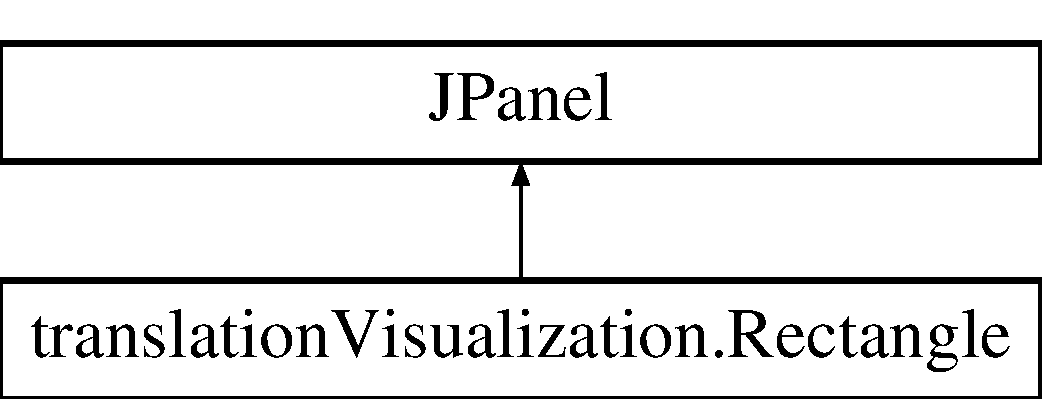
\includegraphics[height=2.000000cm]{classtranslation_visualization_1_1_rectangle}
\end{center}
\end{figure}
\subsection*{Public Member Functions}
\begin{DoxyCompactItemize}
\item 
\mbox{\Hypertarget{classtranslation_visualization_1_1_rectangle_a1f4b83add847f1475ce0cbcfa3410250}\label{classtranslation_visualization_1_1_rectangle_a1f4b83add847f1475ce0cbcfa3410250}} 
List$<$ Point $>$ {\bfseries get\+M\+\_\+\+Region\+Points} ()
\item 
\mbox{\Hypertarget{classtranslation_visualization_1_1_rectangle_a2908d8305e4e4470dc70fb3131d0b3e0}\label{classtranslation_visualization_1_1_rectangle_a2908d8305e4e4470dc70fb3131d0b3e0}} 
void {\bfseries set\+M\+\_\+\+Region\+Points} (List$<$ Point $>$ m\+\_\+\+Region\+Points)
\item 
\mbox{\Hypertarget{classtranslation_visualization_1_1_rectangle_a775207b4d328af2eea2b08c367eded8a}\label{classtranslation_visualization_1_1_rectangle_a775207b4d328af2eea2b08c367eded8a}} 
Point {\bfseries get\+M\+\_\+\+Rect\+Point} ()
\item 
void \hyperlink{classtranslation_visualization_1_1_rectangle_a7f86b7e90bb52bb39d18e4f39ff29f6f}{set\+M\+\_\+\+Rect\+Point} (Point string\+Point)
\item 
\mbox{\Hypertarget{classtranslation_visualization_1_1_rectangle_aaa4f1b231cf0411d5c0257ee04a2b6cc}\label{classtranslation_visualization_1_1_rectangle_aaa4f1b231cf0411d5c0257ee04a2b6cc}} 
int {\bfseries get\+M\+\_\+\+Rect\+Width} ()
\item 
void \hyperlink{classtranslation_visualization_1_1_rectangle_ab6bedb4ab9dc6e6a6baf8e4b0685dd67}{set\+M\+\_\+\+Rect\+Width} (int word\+Frequency)
\item 
\mbox{\Hypertarget{classtranslation_visualization_1_1_rectangle_afec0d7bb7a4db7a5f31faab44f4c1983}\label{classtranslation_visualization_1_1_rectangle_afec0d7bb7a4db7a5f31faab44f4c1983}} 
Color {\bfseries get\+M\+\_\+\+Rect\+Color} ()
\item 
\mbox{\Hypertarget{classtranslation_visualization_1_1_rectangle_a05d272d32a0825b6e5e2cac52f4ea0ea}\label{classtranslation_visualization_1_1_rectangle_a05d272d32a0825b6e5e2cac52f4ea0ea}} 
void {\bfseries set\+M\+\_\+\+Rect\+Color} (Color m\+\_\+\+Rect\+Color)
\item 
\mbox{\Hypertarget{classtranslation_visualization_1_1_rectangle_ab74ebe8a3d1b79adaf0bde29eb9be11a}\label{classtranslation_visualization_1_1_rectangle_ab74ebe8a3d1b79adaf0bde29eb9be11a}} 
int {\bfseries get\+M\+\_\+\+Rect\+Height} ()
\item 
\mbox{\Hypertarget{classtranslation_visualization_1_1_rectangle_ac98a5616a97d39463014ab3670f1662d}\label{classtranslation_visualization_1_1_rectangle_ac98a5616a97d39463014ab3670f1662d}} 
Point {\bfseries get\+M\+\_\+\+Range\+End\+Point} ()
\item 
\mbox{\Hypertarget{classtranslation_visualization_1_1_rectangle_af9a60d975b1bb3023e16a9cf44f9d6d0}\label{classtranslation_visualization_1_1_rectangle_af9a60d975b1bb3023e16a9cf44f9d6d0}} 
void {\bfseries set\+M\+\_\+\+Range\+End\+Point} (Point rect\+Point, int rect\+Height, int rect\+Width)
\end{DoxyCompactItemize}


\subsection{Member Function Documentation}
\mbox{\Hypertarget{classtranslation_visualization_1_1_rectangle_a7f86b7e90bb52bb39d18e4f39ff29f6f}\label{classtranslation_visualization_1_1_rectangle_a7f86b7e90bb52bb39d18e4f39ff29f6f}} 
\index{translation\+Visualization\+::\+Rectangle@{translation\+Visualization\+::\+Rectangle}!set\+M\+\_\+\+Rect\+Point@{set\+M\+\_\+\+Rect\+Point}}
\index{set\+M\+\_\+\+Rect\+Point@{set\+M\+\_\+\+Rect\+Point}!translation\+Visualization\+::\+Rectangle@{translation\+Visualization\+::\+Rectangle}}
\subsubsection{\texorpdfstring{set\+M\+\_\+\+Rect\+Point()}{setM\_RectPoint()}}
{\footnotesize\ttfamily void translation\+Visualization.\+Rectangle.\+set\+M\+\_\+\+Rect\+Point (\begin{DoxyParamCaption}\item[{Point}]{string\+Point }\end{DoxyParamCaption})\hspace{0.3cm}{\ttfamily [inline]}}

Pass the point of string to \hyperlink{classtranslation_visualization_1_1_item}{Item} object and calculate location 
\begin{DoxyParams}{Parameters}
{\em string\+Point} & \\
\hline
\end{DoxyParams}
\mbox{\Hypertarget{classtranslation_visualization_1_1_rectangle_ab6bedb4ab9dc6e6a6baf8e4b0685dd67}\label{classtranslation_visualization_1_1_rectangle_ab6bedb4ab9dc6e6a6baf8e4b0685dd67}} 
\index{translation\+Visualization\+::\+Rectangle@{translation\+Visualization\+::\+Rectangle}!set\+M\+\_\+\+Rect\+Width@{set\+M\+\_\+\+Rect\+Width}}
\index{set\+M\+\_\+\+Rect\+Width@{set\+M\+\_\+\+Rect\+Width}!translation\+Visualization\+::\+Rectangle@{translation\+Visualization\+::\+Rectangle}}
\subsubsection{\texorpdfstring{set\+M\+\_\+\+Rect\+Width()}{setM\_RectWidth()}}
{\footnotesize\ttfamily void translation\+Visualization.\+Rectangle.\+set\+M\+\_\+\+Rect\+Width (\begin{DoxyParamCaption}\item[{int}]{word\+Frequency }\end{DoxyParamCaption})\hspace{0.3cm}{\ttfamily [inline]}}

Pass the frequency number to compute the width of rectangle 
\begin{DoxyParams}{Parameters}
{\em word\+Frequency} & \\
\hline
\end{DoxyParams}


The documentation for this class was generated from the following file\+:\begin{DoxyCompactItemize}
\item 
Rectangle.\+java\end{DoxyCompactItemize}

\hypertarget{classtranslation_visualization_1_1_t_f_i_d_f_calculator}{}\section{translation\+Visualization.\+T\+F\+I\+D\+F\+Calculator Class Reference}
\label{classtranslation_visualization_1_1_t_f_i_d_f_calculator}\index{translation\+Visualization.\+T\+F\+I\+D\+F\+Calculator@{translation\+Visualization.\+T\+F\+I\+D\+F\+Calculator}}
\subsection*{Public Member Functions}
\begin{DoxyCompactItemize}
\item 
\mbox{\Hypertarget{classtranslation_visualization_1_1_t_f_i_d_f_calculator_a1881598c99aeace13b7922c69edda980}\label{classtranslation_visualization_1_1_t_f_i_d_f_calculator_a1881598c99aeace13b7922c69edda980}} 
List$<$ Hashtable$<$ String, Integer $>$ $>$ {\bfseries get\+Lists} ()
\item 
\mbox{\Hypertarget{classtranslation_visualization_1_1_t_f_i_d_f_calculator_aeeeb099a394fb2cb7c935c9f544bd303}\label{classtranslation_visualization_1_1_t_f_i_d_f_calculator_aeeeb099a394fb2cb7c935c9f544bd303}} 
\hyperlink{classtranslation_visualization_1_1_item}{Item} {\bfseries get\+Concordance} ()
\item 
\mbox{\Hypertarget{classtranslation_visualization_1_1_t_f_i_d_f_calculator_ac16eeafdf9eb60f960a3a09c10368d0a}\label{classtranslation_visualization_1_1_t_f_i_d_f_calculator_ac16eeafdf9eb60f960a3a09c10368d0a}} 
void {\bfseries set\+Concordance} (\hyperlink{classtranslation_visualization_1_1_item}{Item} item)
\item 
\mbox{\Hypertarget{classtranslation_visualization_1_1_t_f_i_d_f_calculator_a284d7de1902d3fef52c11e448c08dd8e}\label{classtranslation_visualization_1_1_t_f_i_d_f_calculator_a284d7de1902d3fef52c11e448c08dd8e}} 
Hashtable$<$ String, Integer $>$ {\bfseries get\+Tfidf\+List} ()
\item 
\mbox{\Hypertarget{classtranslation_visualization_1_1_t_f_i_d_f_calculator_a79ac5963ad3479bfcccfcbf5f07ab45b}\label{classtranslation_visualization_1_1_t_f_i_d_f_calculator_a79ac5963ad3479bfcccfcbf5f07ab45b}} 
void {\bfseries set\+Tfidf\+List} (Hashtable$<$ String, Integer $>$ tfidf\+List)
\item 
\mbox{\Hypertarget{classtranslation_visualization_1_1_t_f_i_d_f_calculator_a3f779c17eab4b2cff9b07a097e5574e0}\label{classtranslation_visualization_1_1_t_f_i_d_f_calculator_a3f779c17eab4b2cff9b07a097e5574e0}} 
List$<$ Map.\+Entry$<$ String, Integer $>$ $>$ {\bfseries get\+One\+Doc} ()
\item 
\mbox{\Hypertarget{classtranslation_visualization_1_1_t_f_i_d_f_calculator_a64251c1bdf686853c836ba6f34624164}\label{classtranslation_visualization_1_1_t_f_i_d_f_calculator_a64251c1bdf686853c836ba6f34624164}} 
void {\bfseries set\+One\+Doc} (List$<$ Map.\+Entry$<$ String, Integer $>$$>$ one\+Doc)
\item 
\mbox{\Hypertarget{classtranslation_visualization_1_1_t_f_i_d_f_calculator_a8123f80fe4f52c0ebe64de416850b732}\label{classtranslation_visualization_1_1_t_f_i_d_f_calculator_a8123f80fe4f52c0ebe64de416850b732}} 
List$<$ Hashtable$<$ String, Integer $>$ $>$ {\bfseries initiate} (List$<$ Hashtable$<$ String, Integer $>$$>$ documents)
\item 
double \hyperlink{classtranslation_visualization_1_1_t_f_i_d_f_calculator_ad2d8c3cea991e56ac2c25dee58a65f07}{idf} (List$<$ Hashtable$<$ String, Integer $>$$>$ documents, String term)
\end{DoxyCompactItemize}


\subsection{Detailed Description}
\begin{DoxyAuthor}{Author}
Mohamed Guendouz 
\end{DoxyAuthor}


\subsection{Member Function Documentation}
\mbox{\Hypertarget{classtranslation_visualization_1_1_t_f_i_d_f_calculator_ad2d8c3cea991e56ac2c25dee58a65f07}\label{classtranslation_visualization_1_1_t_f_i_d_f_calculator_ad2d8c3cea991e56ac2c25dee58a65f07}} 
\index{translation\+Visualization\+::\+T\+F\+I\+D\+F\+Calculator@{translation\+Visualization\+::\+T\+F\+I\+D\+F\+Calculator}!idf@{idf}}
\index{idf@{idf}!translation\+Visualization\+::\+T\+F\+I\+D\+F\+Calculator@{translation\+Visualization\+::\+T\+F\+I\+D\+F\+Calculator}}
\subsubsection{\texorpdfstring{idf()}{idf()}}
{\footnotesize\ttfamily double translation\+Visualization.\+T\+F\+I\+D\+F\+Calculator.\+idf (\begin{DoxyParamCaption}\item[{List$<$ Hashtable$<$ String, Integer $>$$>$}]{documents,  }\item[{String}]{term }\end{DoxyParamCaption})\hspace{0.3cm}{\ttfamily [inline]}}


\begin{DoxyParams}{Parameters}
{\em docs} & list of list of strings represents the dataset \\
\hline
{\em term} & String represents a term \\
\hline
\end{DoxyParams}
\begin{DoxyReturn}{Returns}
the inverse term frequency of term in documents 
\end{DoxyReturn}


The documentation for this class was generated from the following file\+:\begin{DoxyCompactItemize}
\item 
T\+F\+I\+D\+F\+Calculator.\+java\end{DoxyCompactItemize}

\hypertarget{classtranslation_visualization_1_1_translation_visualization}{}\section{translation\+Visualization.\+Translation\+Visualization Class Reference}
\label{classtranslation_visualization_1_1_translation_visualization}\index{translation\+Visualization.\+Translation\+Visualization@{translation\+Visualization.\+Translation\+Visualization}}
\subsection*{Public Member Functions}
\begin{DoxyCompactItemize}
\item 
\mbox{\Hypertarget{classtranslation_visualization_1_1_translation_visualization_a3b8103061db8a490b5a82e648a4e6c72}\label{classtranslation_visualization_1_1_translation_visualization_a3b8103061db8a490b5a82e648a4e6c72}} 
String {\bfseries get\+Frame\+Title} ()
\item 
\mbox{\Hypertarget{classtranslation_visualization_1_1_translation_visualization_ad4ec1b5698ba4c099d5c995c384c6acd}\label{classtranslation_visualization_1_1_translation_visualization_ad4ec1b5698ba4c099d5c995c384c6acd}} 
void {\bfseries set\+Frame\+Title} (String frame\+Title)
\item 
\mbox{\Hypertarget{classtranslation_visualization_1_1_translation_visualization_ab441b4354b1393c2cdd755758cfda9f6}\label{classtranslation_visualization_1_1_translation_visualization_ab441b4354b1393c2cdd755758cfda9f6}} 
J\+Button {\bfseries get\+M\+\_\+lemma\+Button} ()
\item 
\mbox{\Hypertarget{classtranslation_visualization_1_1_translation_visualization_a95d88d464799023c0fa82b4e10838fbd}\label{classtranslation_visualization_1_1_translation_visualization_a95d88d464799023c0fa82b4e10838fbd}} 
void {\bfseries set\+M\+\_\+lemma\+Button} (J\+Button m\+\_\+lemma\+Button)
\item 
\mbox{\Hypertarget{classtranslation_visualization_1_1_translation_visualization_a83bcf9e54b9b997e4db120683baebde4}\label{classtranslation_visualization_1_1_translation_visualization_a83bcf9e54b9b997e4db120683baebde4}} 
J\+Button {\bfseries get\+M\+\_\+\+Tf\+Idf\+Button} ()
\item 
\mbox{\Hypertarget{classtranslation_visualization_1_1_translation_visualization_a9c9512d86dd40366ca5d36cd737d986d}\label{classtranslation_visualization_1_1_translation_visualization_a9c9512d86dd40366ca5d36cd737d986d}} 
void {\bfseries set\+M\+\_\+\+Tf\+Idf\+Button} (J\+Button m\+\_\+\+Tf\+Idf\+Button)
\item 
\mbox{\Hypertarget{classtranslation_visualization_1_1_translation_visualization_a3a0efff15b1499827f6e7bbae2fca7b9}\label{classtranslation_visualization_1_1_translation_visualization_a3a0efff15b1499827f6e7bbae2fca7b9}} 
J\+Toggle\+Button {\bfseries get\+M\+\_\+\+Text\+On\+Off\+Button} ()
\item 
\mbox{\Hypertarget{classtranslation_visualization_1_1_translation_visualization_a8d165c8742d9c65457eb3e429763e3dd}\label{classtranslation_visualization_1_1_translation_visualization_a8d165c8742d9c65457eb3e429763e3dd}} 
void {\bfseries set\+M\+\_\+\+Text\+On\+Off\+Button} (J\+Toggle\+Button m\+\_\+\+Text\+On\+Off\+Button)
\item 
\mbox{\Hypertarget{classtranslation_visualization_1_1_translation_visualization_a83ee145d73390c55b9e90eec1106baa5}\label{classtranslation_visualization_1_1_translation_visualization_a83ee145d73390c55b9e90eec1106baa5}} 
J\+Label {\bfseries get\+M\+\_\+\+Slider\+Label} ()
\item 
void \hyperlink{classtranslation_visualization_1_1_translation_visualization_a44e755307d86eca9062b3f796dbf5e15}{set\+M\+\_\+\+Slider\+Label} (J\+Label m\+\_\+\+Slider\+Label, String string)
\item 
\mbox{\Hypertarget{classtranslation_visualization_1_1_translation_visualization_ae4d6cc4b753952eeeae8656fb62a167a}\label{classtranslation_visualization_1_1_translation_visualization_ae4d6cc4b753952eeeae8656fb62a167a}} 
\hyperlink{classtranslation_visualization_1_1_data_reader}{Data\+Reader} {\bfseries get\+Data\+Reader} ()
\item 
\mbox{\Hypertarget{classtranslation_visualization_1_1_translation_visualization_a7ab1999b81f65858d5bd038178f5da61}\label{classtranslation_visualization_1_1_translation_visualization_a7ab1999b81f65858d5bd038178f5da61}} 
void {\bfseries set\+Data\+Reader} (\hyperlink{classtranslation_visualization_1_1_data_reader}{Data\+Reader} data\+Reader)  throws Exception 
\item 
List$<$ \hyperlink{classtranslation_visualization_1_1_version}{Version} $>$ \hyperlink{classtranslation_visualization_1_1_translation_visualization_a6096009fba7843a3aa0f2ee14381cc0f}{get\+Version\+List} ()
\item 
\mbox{\Hypertarget{classtranslation_visualization_1_1_translation_visualization_a96ac36d95f6456e304db20bec920a444}\label{classtranslation_visualization_1_1_translation_visualization_a96ac36d95f6456e304db20bec920a444}} 
void {\bfseries set\+M\+\_\+\+Version\+List} (List$<$ \hyperlink{classtranslation_visualization_1_1_version}{Version} $>$ m\+\_\+\+Version\+List)
\item 
\mbox{\Hypertarget{classtranslation_visualization_1_1_translation_visualization_abf2f9df3311824d335af190a768116ab}\label{classtranslation_visualization_1_1_translation_visualization_abf2f9df3311824d335af190a768116ab}} 
Version\+Chosen\+Panel {\bfseries get\+Version\+Choosing\+Panel} ()
\item 
\mbox{\Hypertarget{classtranslation_visualization_1_1_translation_visualization_a7b4145b39f3594fad08b245cb020b472}\label{classtranslation_visualization_1_1_translation_visualization_a7b4145b39f3594fad08b245cb020b472}} 
void {\bfseries set\+Version\+Choosing\+Panel} (Version\+Chosen\+Panel version\+Choosing\+Panel, Concordance\+Panel concordance\+Panel, List$<$ String $>$ version\+Names)
\item 
J\+Slider \hyperlink{classtranslation_visualization_1_1_translation_visualization_acfa61dfbe046b9340c09b24408002092}{get\+M\+\_\+\+Concordance\+Slider} ()
\item 
void \hyperlink{classtranslation_visualization_1_1_translation_visualization_a1f8a8214bc3e3d76cf4add08e9f49f54}{set\+M\+\_\+\+Concordance\+Slider} ()
\item 
\mbox{\Hypertarget{classtranslation_visualization_1_1_translation_visualization_ae6025a07cb2a10acdc21d6414e37475e}\label{classtranslation_visualization_1_1_translation_visualization_ae6025a07cb2a10acdc21d6414e37475e}} 
J\+Check\+Box {\bfseries get\+Version\+Menu} ()
\item 
J\+Frame \hyperlink{classtranslation_visualization_1_1_translation_visualization_a1d0a60810eb6d9d8dfae70e6f254d519}{get\+Concordance\+Frame} ()
\item 
void \hyperlink{classtranslation_visualization_1_1_translation_visualization_acfd9146c7e934d5788d4dabe0236dd4f}{set\+Concordance\+Frame} (J\+Frame concordance\+Frame)
\item 
\mbox{\Hypertarget{classtranslation_visualization_1_1_translation_visualization_a61655ae18bec032043b797a07f27e410}\label{classtranslation_visualization_1_1_translation_visualization_a61655ae18bec032043b797a07f27e410}} 
J\+Slider {\bfseries get\+M\+\_\+\+Scroll\+Pane\+Slider} ()
\item 
\mbox{\Hypertarget{classtranslation_visualization_1_1_translation_visualization_ae56a89032dbfa85afda7cb839b0f08aa}\label{classtranslation_visualization_1_1_translation_visualization_ae56a89032dbfa85afda7cb839b0f08aa}} 
void {\bfseries set\+M\+\_\+\+Scroll\+Pane\+Slider} ()
\item 
\mbox{\Hypertarget{classtranslation_visualization_1_1_translation_visualization_a8b8444dad889ddc72169db2d37b66635}\label{classtranslation_visualization_1_1_translation_visualization_a8b8444dad889ddc72169db2d37b66635}} 
J\+Panel {\bfseries get\+M\+\_\+\+Scroll\+Panel} ()
\item 
\mbox{\Hypertarget{classtranslation_visualization_1_1_translation_visualization_a9604e2396e518903eb7804371d624725}\label{classtranslation_visualization_1_1_translation_visualization_a9604e2396e518903eb7804371d624725}} 
void {\bfseries set\+M\+\_\+\+Scroll\+Panel} (J\+Panel m\+\_\+\+Scroll\+Panel)
\item 
J\+Scroll\+Pane \hyperlink{classtranslation_visualization_1_1_translation_visualization_a48b65737bbc678d3d8bb5d18d16aa8b4}{get\+Scroll\+Pane} ()
\item 
void \hyperlink{classtranslation_visualization_1_1_translation_visualization_aa47fe2442c918ddf07a4d652aa452c2e}{set\+Scroll\+Pane} (J\+Scroll\+Pane scroll\+Panel)
\item 
J\+Button \hyperlink{classtranslation_visualization_1_1_translation_visualization_a32cb8b84921e6cb4e60546f487c4f178}{get\+Concordance\+Button} ()
\item 
void \hyperlink{classtranslation_visualization_1_1_translation_visualization_ae58f071059815461bf7fa76f08ffba1a}{set\+Concordance\+Button} (J\+Button concordance\+Button)
\item 
J\+Panel \hyperlink{classtranslation_visualization_1_1_translation_visualization_a2b39bd3900687d999084d68fc2594b97}{get\+M\+\_\+visuallization\+Panel} ()
\item 
void \hyperlink{classtranslation_visualization_1_1_translation_visualization_a044c4d17c8fb424e0ebd6cffa215f1d7}{set\+M\+\_\+visuallization\+Panel} (J\+Panel m\+\_\+visuallization\+Panel)
\item 
J\+Panel \hyperlink{classtranslation_visualization_1_1_translation_visualization_a5b90b2e6d17b9d84a57276e8a7b7f6c0}{get\+M\+\_\+\+User\+Option\+Panel} ()
\item 
void \hyperlink{classtranslation_visualization_1_1_translation_visualization_af88ee9e4607e9b967d5676718eec1e7d}{set\+M\+\_\+\+User\+Option\+Panel} (J\+Panel button\+Panel)
\item 
Color\+Legend\+Panel \hyperlink{classtranslation_visualization_1_1_translation_visualization_a6f2ac790f4247e0706fa9b51cf8e24d6}{get\+M\+\_\+\+Color\+Legend\+Panel} ()
\item 
void \hyperlink{classtranslation_visualization_1_1_translation_visualization_aa101a9495f44afc16f938cf13a6f2e24}{set\+M\+\_\+\+Color\+Legend\+Panel} (Color\+Legend\+Panel color\+Legend\+Panel, \hyperlink{classtranslation_visualization_1_1_data_reader}{Data\+Reader} data\+Reader)
\item 
Concordance\+Panel \hyperlink{classtranslation_visualization_1_1_translation_visualization_ada19dca9e30dcb62a0bff2b6c2d2e4e7}{get\+Concordance\+Panel} ()
\item 
void \hyperlink{classtranslation_visualization_1_1_translation_visualization_a55a90cd2c358d5bb4e3a6197180f9a21}{set\+Concordance\+Panel} (Concordance\+Panel concordance\+Panel)
\item 
\mbox{\Hypertarget{classtranslation_visualization_1_1_translation_visualization_a8ca9cdde4b9cc671e37467d8ad37e089}\label{classtranslation_visualization_1_1_translation_visualization_a8ca9cdde4b9cc671e37467d8ad37e089}} 
void {\bfseries set\+Components} ()  throws Exception 
\item 
\mbox{\Hypertarget{classtranslation_visualization_1_1_translation_visualization_a70bb294ec142a9e3d2c3ff8be2dff597}\label{classtranslation_visualization_1_1_translation_visualization_a70bb294ec142a9e3d2c3ff8be2dff597}} 
Grid\+Bag\+Constraints {\bfseries get\+M\+\_\+\+Constraint} ()
\item 
\mbox{\Hypertarget{classtranslation_visualization_1_1_translation_visualization_ae9d30e6e792e39ca6c71803864324602}\label{classtranslation_visualization_1_1_translation_visualization_ae9d30e6e792e39ca6c71803864324602}} 
void {\bfseries set\+M\+\_\+\+Constraint} (int gridx, int gridy, int weightx, int weighty)
\item 
\mbox{\Hypertarget{classtranslation_visualization_1_1_translation_visualization_af7bdd0a31d42d8ff3b6635273272eeaf}\label{classtranslation_visualization_1_1_translation_visualization_af7bdd0a31d42d8ff3b6635273272eeaf}} 
Grid\+Bag\+Layout {\bfseries get\+M\+\_\+\+Panel\+Layout} ()
\item 
\mbox{\Hypertarget{classtranslation_visualization_1_1_translation_visualization_a32b219727c16edd968323bea9e5c1ac1}\label{classtranslation_visualization_1_1_translation_visualization_a32b219727c16edd968323bea9e5c1ac1}} 
void {\bfseries set\+M\+\_\+\+Panel\+Layout} (Grid\+Bag\+Layout m\+\_\+\+Panel\+Layout)
\item 
\mbox{\Hypertarget{classtranslation_visualization_1_1_translation_visualization_afecb35a905797e63be4b194eb7485341}\label{classtranslation_visualization_1_1_translation_visualization_afecb35a905797e63be4b194eb7485341}} 
void {\bfseries initiate\+Vis\+Panel} ()
\item 
\mbox{\Hypertarget{classtranslation_visualization_1_1_translation_visualization_a1078bb3aab15d2905f638f4cba6657c5}\label{classtranslation_visualization_1_1_translation_visualization_a1078bb3aab15d2905f638f4cba6657c5}} 
void {\bfseries initiate\+Trans\+Vis} ()  throws Exception
\item 
\mbox{\Hypertarget{classtranslation_visualization_1_1_translation_visualization_ae44f6548d9d1c4f9986b229f1ba4c639}\label{classtranslation_visualization_1_1_translation_visualization_ae44f6548d9d1c4f9986b229f1ba4c639}} 
void {\bfseries initiate\+User\+Opt\+Panel} ()
\item 
\mbox{\Hypertarget{classtranslation_visualization_1_1_translation_visualization_aaf49f095e96b880086d5bfab853fdca3}\label{classtranslation_visualization_1_1_translation_visualization_aaf49f095e96b880086d5bfab853fdca3}} 
void {\bfseries initiate\+Frame} ()
\end{DoxyCompactItemize}


\subsection{Member Function Documentation}
\mbox{\Hypertarget{classtranslation_visualization_1_1_translation_visualization_a32cb8b84921e6cb4e60546f487c4f178}\label{classtranslation_visualization_1_1_translation_visualization_a32cb8b84921e6cb4e60546f487c4f178}} 
\index{translation\+Visualization\+::\+Translation\+Visualization@{translation\+Visualization\+::\+Translation\+Visualization}!get\+Concordance\+Button@{get\+Concordance\+Button}}
\index{get\+Concordance\+Button@{get\+Concordance\+Button}!translation\+Visualization\+::\+Translation\+Visualization@{translation\+Visualization\+::\+Translation\+Visualization}}
\subsubsection{\texorpdfstring{get\+Concordance\+Button()}{getConcordanceButton()}}
{\footnotesize\ttfamily J\+Button translation\+Visualization.\+Translation\+Visualization.\+get\+Concordance\+Button (\begin{DoxyParamCaption}{ }\end{DoxyParamCaption})\hspace{0.3cm}{\ttfamily [inline]}}

Use this method to access m\+\_\+\+Concordance\+Button

\begin{DoxyReturn}{Returns}
m\+\_\+\+Concordance\+Button 
\end{DoxyReturn}
\mbox{\Hypertarget{classtranslation_visualization_1_1_translation_visualization_a1d0a60810eb6d9d8dfae70e6f254d519}\label{classtranslation_visualization_1_1_translation_visualization_a1d0a60810eb6d9d8dfae70e6f254d519}} 
\index{translation\+Visualization\+::\+Translation\+Visualization@{translation\+Visualization\+::\+Translation\+Visualization}!get\+Concordance\+Frame@{get\+Concordance\+Frame}}
\index{get\+Concordance\+Frame@{get\+Concordance\+Frame}!translation\+Visualization\+::\+Translation\+Visualization@{translation\+Visualization\+::\+Translation\+Visualization}}
\subsubsection{\texorpdfstring{get\+Concordance\+Frame()}{getConcordanceFrame()}}
{\footnotesize\ttfamily J\+Frame translation\+Visualization.\+Translation\+Visualization.\+get\+Concordance\+Frame (\begin{DoxyParamCaption}{ }\end{DoxyParamCaption})\hspace{0.3cm}{\ttfamily [inline]}}

Use this method to access m\+\_\+\+Concordance\+Frame

\begin{DoxyReturn}{Returns}
m\+\_\+\+Concordance\+Frame 
\end{DoxyReturn}
\mbox{\Hypertarget{classtranslation_visualization_1_1_translation_visualization_ada19dca9e30dcb62a0bff2b6c2d2e4e7}\label{classtranslation_visualization_1_1_translation_visualization_ada19dca9e30dcb62a0bff2b6c2d2e4e7}} 
\index{translation\+Visualization\+::\+Translation\+Visualization@{translation\+Visualization\+::\+Translation\+Visualization}!get\+Concordance\+Panel@{get\+Concordance\+Panel}}
\index{get\+Concordance\+Panel@{get\+Concordance\+Panel}!translation\+Visualization\+::\+Translation\+Visualization@{translation\+Visualization\+::\+Translation\+Visualization}}
\subsubsection{\texorpdfstring{get\+Concordance\+Panel()}{getConcordancePanel()}}
{\footnotesize\ttfamily Concordance\+Panel translation\+Visualization.\+Translation\+Visualization.\+get\+Concordance\+Panel (\begin{DoxyParamCaption}{ }\end{DoxyParamCaption})\hspace{0.3cm}{\ttfamily [inline]}}

Use this method to access m\+\_\+\+Concordance\+Panel

\begin{DoxyReturn}{Returns}
m\+\_\+\+Concordance\+Panel 
\end{DoxyReturn}
\mbox{\Hypertarget{classtranslation_visualization_1_1_translation_visualization_a6f2ac790f4247e0706fa9b51cf8e24d6}\label{classtranslation_visualization_1_1_translation_visualization_a6f2ac790f4247e0706fa9b51cf8e24d6}} 
\index{translation\+Visualization\+::\+Translation\+Visualization@{translation\+Visualization\+::\+Translation\+Visualization}!get\+M\+\_\+\+Color\+Legend\+Panel@{get\+M\+\_\+\+Color\+Legend\+Panel}}
\index{get\+M\+\_\+\+Color\+Legend\+Panel@{get\+M\+\_\+\+Color\+Legend\+Panel}!translation\+Visualization\+::\+Translation\+Visualization@{translation\+Visualization\+::\+Translation\+Visualization}}
\subsubsection{\texorpdfstring{get\+M\+\_\+\+Color\+Legend\+Panel()}{getM\_ColorLegendPanel()}}
{\footnotesize\ttfamily Color\+Legend\+Panel translation\+Visualization.\+Translation\+Visualization.\+get\+M\+\_\+\+Color\+Legend\+Panel (\begin{DoxyParamCaption}{ }\end{DoxyParamCaption})\hspace{0.3cm}{\ttfamily [inline]}}

Use this method to access m\+\_\+\+Color\+Legend\+Panel

\begin{DoxyReturn}{Returns}
m\+\_\+\+Color\+Legend\+Panel 
\end{DoxyReturn}
\mbox{\Hypertarget{classtranslation_visualization_1_1_translation_visualization_acfa61dfbe046b9340c09b24408002092}\label{classtranslation_visualization_1_1_translation_visualization_acfa61dfbe046b9340c09b24408002092}} 
\index{translation\+Visualization\+::\+Translation\+Visualization@{translation\+Visualization\+::\+Translation\+Visualization}!get\+M\+\_\+\+Concordance\+Slider@{get\+M\+\_\+\+Concordance\+Slider}}
\index{get\+M\+\_\+\+Concordance\+Slider@{get\+M\+\_\+\+Concordance\+Slider}!translation\+Visualization\+::\+Translation\+Visualization@{translation\+Visualization\+::\+Translation\+Visualization}}
\subsubsection{\texorpdfstring{get\+M\+\_\+\+Concordance\+Slider()}{getM\_ConcordanceSlider()}}
{\footnotesize\ttfamily J\+Slider translation\+Visualization.\+Translation\+Visualization.\+get\+M\+\_\+\+Concordance\+Slider (\begin{DoxyParamCaption}{ }\end{DoxyParamCaption})\hspace{0.3cm}{\ttfamily [inline]}}

Use this method to access m\+\_\+\+Concordance\+Slider

\begin{DoxyReturn}{Returns}
m\+\_\+\+Concordance\+Slider 
\end{DoxyReturn}
\mbox{\Hypertarget{classtranslation_visualization_1_1_translation_visualization_a5b90b2e6d17b9d84a57276e8a7b7f6c0}\label{classtranslation_visualization_1_1_translation_visualization_a5b90b2e6d17b9d84a57276e8a7b7f6c0}} 
\index{translation\+Visualization\+::\+Translation\+Visualization@{translation\+Visualization\+::\+Translation\+Visualization}!get\+M\+\_\+\+User\+Option\+Panel@{get\+M\+\_\+\+User\+Option\+Panel}}
\index{get\+M\+\_\+\+User\+Option\+Panel@{get\+M\+\_\+\+User\+Option\+Panel}!translation\+Visualization\+::\+Translation\+Visualization@{translation\+Visualization\+::\+Translation\+Visualization}}
\subsubsection{\texorpdfstring{get\+M\+\_\+\+User\+Option\+Panel()}{getM\_UserOptionPanel()}}
{\footnotesize\ttfamily J\+Panel translation\+Visualization.\+Translation\+Visualization.\+get\+M\+\_\+\+User\+Option\+Panel (\begin{DoxyParamCaption}{ }\end{DoxyParamCaption})\hspace{0.3cm}{\ttfamily [inline]}}

Use this method to access m\+\_\+button\+Panel

\begin{DoxyReturn}{Returns}
m\+\_\+button\+Panel 
\end{DoxyReturn}
\mbox{\Hypertarget{classtranslation_visualization_1_1_translation_visualization_a2b39bd3900687d999084d68fc2594b97}\label{classtranslation_visualization_1_1_translation_visualization_a2b39bd3900687d999084d68fc2594b97}} 
\index{translation\+Visualization\+::\+Translation\+Visualization@{translation\+Visualization\+::\+Translation\+Visualization}!get\+M\+\_\+visuallization\+Panel@{get\+M\+\_\+visuallization\+Panel}}
\index{get\+M\+\_\+visuallization\+Panel@{get\+M\+\_\+visuallization\+Panel}!translation\+Visualization\+::\+Translation\+Visualization@{translation\+Visualization\+::\+Translation\+Visualization}}
\subsubsection{\texorpdfstring{get\+M\+\_\+visuallization\+Panel()}{getM\_visuallizationPanel()}}
{\footnotesize\ttfamily J\+Panel translation\+Visualization.\+Translation\+Visualization.\+get\+M\+\_\+visuallization\+Panel (\begin{DoxyParamCaption}{ }\end{DoxyParamCaption})\hspace{0.3cm}{\ttfamily [inline]}}

Use this method to access m\+\_\+visuallization\+Panel

\begin{DoxyReturn}{Returns}
m\+\_\+visuallization\+Panel 
\end{DoxyReturn}
\mbox{\Hypertarget{classtranslation_visualization_1_1_translation_visualization_a48b65737bbc678d3d8bb5d18d16aa8b4}\label{classtranslation_visualization_1_1_translation_visualization_a48b65737bbc678d3d8bb5d18d16aa8b4}} 
\index{translation\+Visualization\+::\+Translation\+Visualization@{translation\+Visualization\+::\+Translation\+Visualization}!get\+Scroll\+Pane@{get\+Scroll\+Pane}}
\index{get\+Scroll\+Pane@{get\+Scroll\+Pane}!translation\+Visualization\+::\+Translation\+Visualization@{translation\+Visualization\+::\+Translation\+Visualization}}
\subsubsection{\texorpdfstring{get\+Scroll\+Pane()}{getScrollPane()}}
{\footnotesize\ttfamily J\+Scroll\+Pane translation\+Visualization.\+Translation\+Visualization.\+get\+Scroll\+Pane (\begin{DoxyParamCaption}{ }\end{DoxyParamCaption})\hspace{0.3cm}{\ttfamily [inline]}}

Use this method to access m\+\_\+\+Scroll\+Panel

\begin{DoxyReturn}{Returns}
m\+\_\+\+Scroll\+Panel 
\end{DoxyReturn}
\mbox{\Hypertarget{classtranslation_visualization_1_1_translation_visualization_a6096009fba7843a3aa0f2ee14381cc0f}\label{classtranslation_visualization_1_1_translation_visualization_a6096009fba7843a3aa0f2ee14381cc0f}} 
\index{translation\+Visualization\+::\+Translation\+Visualization@{translation\+Visualization\+::\+Translation\+Visualization}!get\+Version\+List@{get\+Version\+List}}
\index{get\+Version\+List@{get\+Version\+List}!translation\+Visualization\+::\+Translation\+Visualization@{translation\+Visualization\+::\+Translation\+Visualization}}
\subsubsection{\texorpdfstring{get\+Version\+List()}{getVersionList()}}
{\footnotesize\ttfamily List$<$\hyperlink{classtranslation_visualization_1_1_version}{Version}$>$ translation\+Visualization.\+Translation\+Visualization.\+get\+Version\+List (\begin{DoxyParamCaption}{ }\end{DoxyParamCaption})\hspace{0.3cm}{\ttfamily [inline]}}

Use this method to access m\+\_\+\+Version\+List

\begin{DoxyReturn}{Returns}
m\+\_\+\+Version\+List 
\end{DoxyReturn}

\begin{DoxyExceptions}{Exceptions}
{\em Exception} & \\
\hline
\end{DoxyExceptions}
\mbox{\Hypertarget{classtranslation_visualization_1_1_translation_visualization_ae58f071059815461bf7fa76f08ffba1a}\label{classtranslation_visualization_1_1_translation_visualization_ae58f071059815461bf7fa76f08ffba1a}} 
\index{translation\+Visualization\+::\+Translation\+Visualization@{translation\+Visualization\+::\+Translation\+Visualization}!set\+Concordance\+Button@{set\+Concordance\+Button}}
\index{set\+Concordance\+Button@{set\+Concordance\+Button}!translation\+Visualization\+::\+Translation\+Visualization@{translation\+Visualization\+::\+Translation\+Visualization}}
\subsubsection{\texorpdfstring{set\+Concordance\+Button()}{setConcordanceButton()}}
{\footnotesize\ttfamily void translation\+Visualization.\+Translation\+Visualization.\+set\+Concordance\+Button (\begin{DoxyParamCaption}\item[{J\+Button}]{concordance\+Button }\end{DoxyParamCaption})\hspace{0.3cm}{\ttfamily [inline]}}

Use this method to create and set m\+\_\+\+Concordance\+Button


\begin{DoxyParams}{Parameters}
{\em concordance\+Button} & \\
\hline
\end{DoxyParams}
\mbox{\Hypertarget{classtranslation_visualization_1_1_translation_visualization_acfd9146c7e934d5788d4dabe0236dd4f}\label{classtranslation_visualization_1_1_translation_visualization_acfd9146c7e934d5788d4dabe0236dd4f}} 
\index{translation\+Visualization\+::\+Translation\+Visualization@{translation\+Visualization\+::\+Translation\+Visualization}!set\+Concordance\+Frame@{set\+Concordance\+Frame}}
\index{set\+Concordance\+Frame@{set\+Concordance\+Frame}!translation\+Visualization\+::\+Translation\+Visualization@{translation\+Visualization\+::\+Translation\+Visualization}}
\subsubsection{\texorpdfstring{set\+Concordance\+Frame()}{setConcordanceFrame()}}
{\footnotesize\ttfamily void translation\+Visualization.\+Translation\+Visualization.\+set\+Concordance\+Frame (\begin{DoxyParamCaption}\item[{J\+Frame}]{concordance\+Frame }\end{DoxyParamCaption})\hspace{0.3cm}{\ttfamily [inline]}}

Use this method to create and set m\+\_\+\+Concordance\+Frame


\begin{DoxyParams}{Parameters}
{\em concordance\+Frame} & \\
\hline
\end{DoxyParams}
\mbox{\Hypertarget{classtranslation_visualization_1_1_translation_visualization_a55a90cd2c358d5bb4e3a6197180f9a21}\label{classtranslation_visualization_1_1_translation_visualization_a55a90cd2c358d5bb4e3a6197180f9a21}} 
\index{translation\+Visualization\+::\+Translation\+Visualization@{translation\+Visualization\+::\+Translation\+Visualization}!set\+Concordance\+Panel@{set\+Concordance\+Panel}}
\index{set\+Concordance\+Panel@{set\+Concordance\+Panel}!translation\+Visualization\+::\+Translation\+Visualization@{translation\+Visualization\+::\+Translation\+Visualization}}
\subsubsection{\texorpdfstring{set\+Concordance\+Panel()}{setConcordancePanel()}}
{\footnotesize\ttfamily void translation\+Visualization.\+Translation\+Visualization.\+set\+Concordance\+Panel (\begin{DoxyParamCaption}\item[{Concordance\+Panel}]{concordance\+Panel }\end{DoxyParamCaption})\hspace{0.3cm}{\ttfamily [inline]}}

Use this method to create and set m\+\_\+\+Concordance\+Panel


\begin{DoxyParams}{Parameters}
{\em concordance\+Panel} & \\
\hline
\end{DoxyParams}
\mbox{\Hypertarget{classtranslation_visualization_1_1_translation_visualization_aa101a9495f44afc16f938cf13a6f2e24}\label{classtranslation_visualization_1_1_translation_visualization_aa101a9495f44afc16f938cf13a6f2e24}} 
\index{translation\+Visualization\+::\+Translation\+Visualization@{translation\+Visualization\+::\+Translation\+Visualization}!set\+M\+\_\+\+Color\+Legend\+Panel@{set\+M\+\_\+\+Color\+Legend\+Panel}}
\index{set\+M\+\_\+\+Color\+Legend\+Panel@{set\+M\+\_\+\+Color\+Legend\+Panel}!translation\+Visualization\+::\+Translation\+Visualization@{translation\+Visualization\+::\+Translation\+Visualization}}
\subsubsection{\texorpdfstring{set\+M\+\_\+\+Color\+Legend\+Panel()}{setM\_ColorLegendPanel()}}
{\footnotesize\ttfamily void translation\+Visualization.\+Translation\+Visualization.\+set\+M\+\_\+\+Color\+Legend\+Panel (\begin{DoxyParamCaption}\item[{Color\+Legend\+Panel}]{color\+Legend\+Panel,  }\item[{\hyperlink{classtranslation_visualization_1_1_data_reader}{Data\+Reader}}]{data\+Reader }\end{DoxyParamCaption})\hspace{0.3cm}{\ttfamily [inline]}}

Use this method to create and set m\+\_\+\+Color\+Legend\+Panel


\begin{DoxyParams}{Parameters}
{\em color\+Legend\+Panel} & \\
\hline
{\em data\+Reader} & \\
\hline
\end{DoxyParams}
\mbox{\Hypertarget{classtranslation_visualization_1_1_translation_visualization_a1f8a8214bc3e3d76cf4add08e9f49f54}\label{classtranslation_visualization_1_1_translation_visualization_a1f8a8214bc3e3d76cf4add08e9f49f54}} 
\index{translation\+Visualization\+::\+Translation\+Visualization@{translation\+Visualization\+::\+Translation\+Visualization}!set\+M\+\_\+\+Concordance\+Slider@{set\+M\+\_\+\+Concordance\+Slider}}
\index{set\+M\+\_\+\+Concordance\+Slider@{set\+M\+\_\+\+Concordance\+Slider}!translation\+Visualization\+::\+Translation\+Visualization@{translation\+Visualization\+::\+Translation\+Visualization}}
\subsubsection{\texorpdfstring{set\+M\+\_\+\+Concordance\+Slider()}{setM\_ConcordanceSlider()}}
{\footnotesize\ttfamily void translation\+Visualization.\+Translation\+Visualization.\+set\+M\+\_\+\+Concordance\+Slider (\begin{DoxyParamCaption}{ }\end{DoxyParamCaption})\hspace{0.3cm}{\ttfamily [inline]}}

Use this method to create and set m\+\_\+\+Concordance\+Slider


\begin{DoxyParams}{Parameters}
{\em m\+\_\+\+Slider} & \\
\hline
\end{DoxyParams}
\mbox{\Hypertarget{classtranslation_visualization_1_1_translation_visualization_a44e755307d86eca9062b3f796dbf5e15}\label{classtranslation_visualization_1_1_translation_visualization_a44e755307d86eca9062b3f796dbf5e15}} 
\index{translation\+Visualization\+::\+Translation\+Visualization@{translation\+Visualization\+::\+Translation\+Visualization}!set\+M\+\_\+\+Slider\+Label@{set\+M\+\_\+\+Slider\+Label}}
\index{set\+M\+\_\+\+Slider\+Label@{set\+M\+\_\+\+Slider\+Label}!translation\+Visualization\+::\+Translation\+Visualization@{translation\+Visualization\+::\+Translation\+Visualization}}
\subsubsection{\texorpdfstring{set\+M\+\_\+\+Slider\+Label()}{setM\_SliderLabel()}}
{\footnotesize\ttfamily void translation\+Visualization.\+Translation\+Visualization.\+set\+M\+\_\+\+Slider\+Label (\begin{DoxyParamCaption}\item[{J\+Label}]{m\+\_\+\+Slider\+Label,  }\item[{String}]{string }\end{DoxyParamCaption})\hspace{0.3cm}{\ttfamily [inline]}}


\begin{DoxyParams}{Parameters}
{\em m\+\_\+\+Slider\+Label} & \\
\hline
{\em string} & \\
\hline
\end{DoxyParams}
\mbox{\Hypertarget{classtranslation_visualization_1_1_translation_visualization_af88ee9e4607e9b967d5676718eec1e7d}\label{classtranslation_visualization_1_1_translation_visualization_af88ee9e4607e9b967d5676718eec1e7d}} 
\index{translation\+Visualization\+::\+Translation\+Visualization@{translation\+Visualization\+::\+Translation\+Visualization}!set\+M\+\_\+\+User\+Option\+Panel@{set\+M\+\_\+\+User\+Option\+Panel}}
\index{set\+M\+\_\+\+User\+Option\+Panel@{set\+M\+\_\+\+User\+Option\+Panel}!translation\+Visualization\+::\+Translation\+Visualization@{translation\+Visualization\+::\+Translation\+Visualization}}
\subsubsection{\texorpdfstring{set\+M\+\_\+\+User\+Option\+Panel()}{setM\_UserOptionPanel()}}
{\footnotesize\ttfamily void translation\+Visualization.\+Translation\+Visualization.\+set\+M\+\_\+\+User\+Option\+Panel (\begin{DoxyParamCaption}\item[{J\+Panel}]{button\+Panel }\end{DoxyParamCaption})\hspace{0.3cm}{\ttfamily [inline]}}

Use this method to create and set m\+\_\+button\+Panel


\begin{DoxyParams}{Parameters}
{\em button\+Panel} & \\
\hline
\end{DoxyParams}
\mbox{\Hypertarget{classtranslation_visualization_1_1_translation_visualization_a044c4d17c8fb424e0ebd6cffa215f1d7}\label{classtranslation_visualization_1_1_translation_visualization_a044c4d17c8fb424e0ebd6cffa215f1d7}} 
\index{translation\+Visualization\+::\+Translation\+Visualization@{translation\+Visualization\+::\+Translation\+Visualization}!set\+M\+\_\+visuallization\+Panel@{set\+M\+\_\+visuallization\+Panel}}
\index{set\+M\+\_\+visuallization\+Panel@{set\+M\+\_\+visuallization\+Panel}!translation\+Visualization\+::\+Translation\+Visualization@{translation\+Visualization\+::\+Translation\+Visualization}}
\subsubsection{\texorpdfstring{set\+M\+\_\+visuallization\+Panel()}{setM\_visuallizationPanel()}}
{\footnotesize\ttfamily void translation\+Visualization.\+Translation\+Visualization.\+set\+M\+\_\+visuallization\+Panel (\begin{DoxyParamCaption}\item[{J\+Panel}]{m\+\_\+visuallization\+Panel }\end{DoxyParamCaption})\hspace{0.3cm}{\ttfamily [inline]}}

Use this method to create and set m\+\_\+visuallization\+Panel


\begin{DoxyParams}{Parameters}
{\em m\+\_\+visuallization\+Panel} & \\
\hline
\end{DoxyParams}
\mbox{\Hypertarget{classtranslation_visualization_1_1_translation_visualization_aa47fe2442c918ddf07a4d652aa452c2e}\label{classtranslation_visualization_1_1_translation_visualization_aa47fe2442c918ddf07a4d652aa452c2e}} 
\index{translation\+Visualization\+::\+Translation\+Visualization@{translation\+Visualization\+::\+Translation\+Visualization}!set\+Scroll\+Pane@{set\+Scroll\+Pane}}
\index{set\+Scroll\+Pane@{set\+Scroll\+Pane}!translation\+Visualization\+::\+Translation\+Visualization@{translation\+Visualization\+::\+Translation\+Visualization}}
\subsubsection{\texorpdfstring{set\+Scroll\+Pane()}{setScrollPane()}}
{\footnotesize\ttfamily void translation\+Visualization.\+Translation\+Visualization.\+set\+Scroll\+Pane (\begin{DoxyParamCaption}\item[{J\+Scroll\+Pane}]{scroll\+Panel }\end{DoxyParamCaption})\hspace{0.3cm}{\ttfamily [inline]}}

Use this method to create and set m\+\_\+\+Scroll\+Panel


\begin{DoxyParams}{Parameters}
{\em scroll\+Panel} & \\
\hline
\end{DoxyParams}


The documentation for this class was generated from the following file\+:\begin{DoxyCompactItemize}
\item 
Translation\+Visualization.\+java\end{DoxyCompactItemize}

\hypertarget{classtranslation_visualization_1_1_version}{}\section{translation\+Visualization.\+Version Class Reference}
\label{classtranslation_visualization_1_1_version}\index{translation\+Visualization.\+Version@{translation\+Visualization.\+Version}}
\subsection*{Public Member Functions}
\begin{DoxyCompactItemize}
\item 
Font \hyperlink{classtranslation_visualization_1_1_version_a00ddc1ca0df8cc633c3a779ee13b81cf}{get\+M\+\_\+\+W\+O\+R\+D\+\_\+\+F\+O\+NT} ()
\item 
List$<$ String $>$ \hyperlink{classtranslation_visualization_1_1_version_acf622708a49469ccb939949106080c12}{get\+M\+\_\+\+Words\+List} ()
\item 
void \hyperlink{classtranslation_visualization_1_1_version_a8c41aeab41d000da67ec2cae090cc105}{set\+M\+\_\+\+Words\+List} (List$<$ String $>$ m\+\_\+\+Words)
\item 
String \hyperlink{classtranslation_visualization_1_1_version_ab54f739831734543ef48d88374b23310}{get\+M\+\_\+\+Version\+Name} ()
\item 
void \hyperlink{classtranslation_visualization_1_1_version_a292cc8922a96f69f299b3eb12e4f6bae}{set\+M\+\_\+\+Version\+Name} (String m\+\_\+\+Version\+Name)
\item 
String \hyperlink{classtranslation_visualization_1_1_version_a122a700e0290511d0fb75bbc16124e3c}{get\+M\+\_\+\+Author} ()
\item 
void \hyperlink{classtranslation_visualization_1_1_version_a01d0c95b99805c6313ec9c32d61566e0}{set\+M\+\_\+\+Author} (String version\+File\+Name)
\item 
int \hyperlink{classtranslation_visualization_1_1_version_a66d8cbf0bbe303e6dd597d1149f5ba1e}{get\+M\+\_\+\+Version\+Number} ()
\item 
void \hyperlink{classtranslation_visualization_1_1_version_a6850428c26c2d1e29ab34042b25a00d5}{set\+M\+\_\+\+Version\+Number} (int m\+\_\+\+Version\+Number)
\item 
int \hyperlink{classtranslation_visualization_1_1_version_a5c63860efc09b62890a595c28a7b9129}{get\+M\+\_\+\+Version\+Year} ()
\item 
void \hyperlink{classtranslation_visualization_1_1_version_a4151be9b0ec9b16a26c2a9ccfc49c69b}{set\+M\+\_\+\+Version\+Year} (String version\+File\+Name)
\item 
\hyperlink{classtranslation_visualization_1_1_item}{Item} \hyperlink{classtranslation_visualization_1_1_version_a02ee5ec71b321d0f425b55c1bf60ade7}{get\+M\+\_\+\+Concordance} ()
\item 
void \hyperlink{classtranslation_visualization_1_1_version_a3e999218715e8099cb6d5de152b20ef4}{set\+M\+\_\+\+Concordance} (\hyperlink{classtranslation_visualization_1_1_item}{Item} m\+\_\+\+Concordance)
\item 
List$<$ \hyperlink{classtranslation_visualization_1_1_item}{Item} $>$ \hyperlink{classtranslation_visualization_1_1_version_a4f18e386beff290d788e426414f62e27}{get\+M\+\_\+\+Concordance\+List} ()
\item 
void \hyperlink{classtranslation_visualization_1_1_version_a5a59a5e66eed9a1087c7a40d8f1f3e9f}{set\+M\+\_\+\+Concordance\+List} (\hyperlink{classtranslation_visualization_1_1_item}{Item} m\+\_\+\+Concordance)
\item 
Point \hyperlink{classtranslation_visualization_1_1_version_a0ff3f88a5e95c7dc3a41dce9f45b7bd6}{get\+M\+\_\+title\+Point} ()
\item 
void \hyperlink{classtranslation_visualization_1_1_version_a90f774c31c131b82dcb57ad1f73d1456}{set\+M\+\_\+title\+Point} (Point point)
\end{DoxyCompactItemize}


\subsection{Member Function Documentation}
\mbox{\Hypertarget{classtranslation_visualization_1_1_version_a122a700e0290511d0fb75bbc16124e3c}\label{classtranslation_visualization_1_1_version_a122a700e0290511d0fb75bbc16124e3c}} 
\index{translation\+Visualization\+::\+Version@{translation\+Visualization\+::\+Version}!get\+M\+\_\+\+Author@{get\+M\+\_\+\+Author}}
\index{get\+M\+\_\+\+Author@{get\+M\+\_\+\+Author}!translation\+Visualization\+::\+Version@{translation\+Visualization\+::\+Version}}
\subsubsection{\texorpdfstring{get\+M\+\_\+\+Author()}{getM\_Author()}}
{\footnotesize\ttfamily String translation\+Visualization.\+Version.\+get\+M\+\_\+\+Author (\begin{DoxyParamCaption}{ }\end{DoxyParamCaption})\hspace{0.3cm}{\ttfamily [inline]}}

\begin{DoxyReturn}{Returns}
author name 
\end{DoxyReturn}
\mbox{\Hypertarget{classtranslation_visualization_1_1_version_a02ee5ec71b321d0f425b55c1bf60ade7}\label{classtranslation_visualization_1_1_version_a02ee5ec71b321d0f425b55c1bf60ade7}} 
\index{translation\+Visualization\+::\+Version@{translation\+Visualization\+::\+Version}!get\+M\+\_\+\+Concordance@{get\+M\+\_\+\+Concordance}}
\index{get\+M\+\_\+\+Concordance@{get\+M\+\_\+\+Concordance}!translation\+Visualization\+::\+Version@{translation\+Visualization\+::\+Version}}
\subsubsection{\texorpdfstring{get\+M\+\_\+\+Concordance()}{getM\_Concordance()}}
{\footnotesize\ttfamily \hyperlink{classtranslation_visualization_1_1_item}{Item} translation\+Visualization.\+Version.\+get\+M\+\_\+\+Concordance (\begin{DoxyParamCaption}{ }\end{DoxyParamCaption})\hspace{0.3cm}{\ttfamily [inline]}}

\begin{DoxyReturn}{Returns}
one concordance 
\end{DoxyReturn}
\mbox{\Hypertarget{classtranslation_visualization_1_1_version_a4f18e386beff290d788e426414f62e27}\label{classtranslation_visualization_1_1_version_a4f18e386beff290d788e426414f62e27}} 
\index{translation\+Visualization\+::\+Version@{translation\+Visualization\+::\+Version}!get\+M\+\_\+\+Concordance\+List@{get\+M\+\_\+\+Concordance\+List}}
\index{get\+M\+\_\+\+Concordance\+List@{get\+M\+\_\+\+Concordance\+List}!translation\+Visualization\+::\+Version@{translation\+Visualization\+::\+Version}}
\subsubsection{\texorpdfstring{get\+M\+\_\+\+Concordance\+List()}{getM\_ConcordanceList()}}
{\footnotesize\ttfamily List$<$\hyperlink{classtranslation_visualization_1_1_item}{Item}$>$ translation\+Visualization.\+Version.\+get\+M\+\_\+\+Concordance\+List (\begin{DoxyParamCaption}{ }\end{DoxyParamCaption})\hspace{0.3cm}{\ttfamily [inline]}}

\begin{DoxyReturn}{Returns}
a list of concordance in current version 
\end{DoxyReturn}
\mbox{\Hypertarget{classtranslation_visualization_1_1_version_a0ff3f88a5e95c7dc3a41dce9f45b7bd6}\label{classtranslation_visualization_1_1_version_a0ff3f88a5e95c7dc3a41dce9f45b7bd6}} 
\index{translation\+Visualization\+::\+Version@{translation\+Visualization\+::\+Version}!get\+M\+\_\+title\+Point@{get\+M\+\_\+title\+Point}}
\index{get\+M\+\_\+title\+Point@{get\+M\+\_\+title\+Point}!translation\+Visualization\+::\+Version@{translation\+Visualization\+::\+Version}}
\subsubsection{\texorpdfstring{get\+M\+\_\+title\+Point()}{getM\_titlePoint()}}
{\footnotesize\ttfamily Point translation\+Visualization.\+Version.\+get\+M\+\_\+title\+Point (\begin{DoxyParamCaption}{ }\end{DoxyParamCaption})\hspace{0.3cm}{\ttfamily [inline]}}

\begin{DoxyReturn}{Returns}
the location point of version title 
\end{DoxyReturn}
\mbox{\Hypertarget{classtranslation_visualization_1_1_version_ab54f739831734543ef48d88374b23310}\label{classtranslation_visualization_1_1_version_ab54f739831734543ef48d88374b23310}} 
\index{translation\+Visualization\+::\+Version@{translation\+Visualization\+::\+Version}!get\+M\+\_\+\+Version\+Name@{get\+M\+\_\+\+Version\+Name}}
\index{get\+M\+\_\+\+Version\+Name@{get\+M\+\_\+\+Version\+Name}!translation\+Visualization\+::\+Version@{translation\+Visualization\+::\+Version}}
\subsubsection{\texorpdfstring{get\+M\+\_\+\+Version\+Name()}{getM\_VersionName()}}
{\footnotesize\ttfamily String translation\+Visualization.\+Version.\+get\+M\+\_\+\+Version\+Name (\begin{DoxyParamCaption}{ }\end{DoxyParamCaption})\hspace{0.3cm}{\ttfamily [inline]}}

\begin{DoxyReturn}{Returns}
version name 
\end{DoxyReturn}
\mbox{\Hypertarget{classtranslation_visualization_1_1_version_a66d8cbf0bbe303e6dd597d1149f5ba1e}\label{classtranslation_visualization_1_1_version_a66d8cbf0bbe303e6dd597d1149f5ba1e}} 
\index{translation\+Visualization\+::\+Version@{translation\+Visualization\+::\+Version}!get\+M\+\_\+\+Version\+Number@{get\+M\+\_\+\+Version\+Number}}
\index{get\+M\+\_\+\+Version\+Number@{get\+M\+\_\+\+Version\+Number}!translation\+Visualization\+::\+Version@{translation\+Visualization\+::\+Version}}
\subsubsection{\texorpdfstring{get\+M\+\_\+\+Version\+Number()}{getM\_VersionNumber()}}
{\footnotesize\ttfamily int translation\+Visualization.\+Version.\+get\+M\+\_\+\+Version\+Number (\begin{DoxyParamCaption}{ }\end{DoxyParamCaption})\hspace{0.3cm}{\ttfamily [inline]}}

\begin{DoxyReturn}{Returns}
the number of version 
\end{DoxyReturn}
\mbox{\Hypertarget{classtranslation_visualization_1_1_version_a5c63860efc09b62890a595c28a7b9129}\label{classtranslation_visualization_1_1_version_a5c63860efc09b62890a595c28a7b9129}} 
\index{translation\+Visualization\+::\+Version@{translation\+Visualization\+::\+Version}!get\+M\+\_\+\+Version\+Year@{get\+M\+\_\+\+Version\+Year}}
\index{get\+M\+\_\+\+Version\+Year@{get\+M\+\_\+\+Version\+Year}!translation\+Visualization\+::\+Version@{translation\+Visualization\+::\+Version}}
\subsubsection{\texorpdfstring{get\+M\+\_\+\+Version\+Year()}{getM\_VersionYear()}}
{\footnotesize\ttfamily int translation\+Visualization.\+Version.\+get\+M\+\_\+\+Version\+Year (\begin{DoxyParamCaption}{ }\end{DoxyParamCaption})\hspace{0.3cm}{\ttfamily [inline]}}

\begin{DoxyReturn}{Returns}
the version year 
\end{DoxyReturn}
\mbox{\Hypertarget{classtranslation_visualization_1_1_version_a00ddc1ca0df8cc633c3a779ee13b81cf}\label{classtranslation_visualization_1_1_version_a00ddc1ca0df8cc633c3a779ee13b81cf}} 
\index{translation\+Visualization\+::\+Version@{translation\+Visualization\+::\+Version}!get\+M\+\_\+\+W\+O\+R\+D\+\_\+\+F\+O\+NT@{get\+M\+\_\+\+W\+O\+R\+D\+\_\+\+F\+O\+NT}}
\index{get\+M\+\_\+\+W\+O\+R\+D\+\_\+\+F\+O\+NT@{get\+M\+\_\+\+W\+O\+R\+D\+\_\+\+F\+O\+NT}!translation\+Visualization\+::\+Version@{translation\+Visualization\+::\+Version}}
\subsubsection{\texorpdfstring{get\+M\+\_\+\+W\+O\+R\+D\+\_\+\+F\+O\+N\+T()}{getM\_WORD\_FONT()}}
{\footnotesize\ttfamily Font translation\+Visualization.\+Version.\+get\+M\+\_\+\+W\+O\+R\+D\+\_\+\+F\+O\+NT (\begin{DoxyParamCaption}{ }\end{DoxyParamCaption})\hspace{0.3cm}{\ttfamily [inline]}}

\begin{DoxyReturn}{Returns}
the fond of the title 
\end{DoxyReturn}
\mbox{\Hypertarget{classtranslation_visualization_1_1_version_acf622708a49469ccb939949106080c12}\label{classtranslation_visualization_1_1_version_acf622708a49469ccb939949106080c12}} 
\index{translation\+Visualization\+::\+Version@{translation\+Visualization\+::\+Version}!get\+M\+\_\+\+Words\+List@{get\+M\+\_\+\+Words\+List}}
\index{get\+M\+\_\+\+Words\+List@{get\+M\+\_\+\+Words\+List}!translation\+Visualization\+::\+Version@{translation\+Visualization\+::\+Version}}
\subsubsection{\texorpdfstring{get\+M\+\_\+\+Words\+List()}{getM\_WordsList()}}
{\footnotesize\ttfamily List$<$String$>$ translation\+Visualization.\+Version.\+get\+M\+\_\+\+Words\+List (\begin{DoxyParamCaption}{ }\end{DoxyParamCaption})\hspace{0.3cm}{\ttfamily [inline]}}

\begin{DoxyReturn}{Returns}
a list of all tokens in one version 
\end{DoxyReturn}
\mbox{\Hypertarget{classtranslation_visualization_1_1_version_a01d0c95b99805c6313ec9c32d61566e0}\label{classtranslation_visualization_1_1_version_a01d0c95b99805c6313ec9c32d61566e0}} 
\index{translation\+Visualization\+::\+Version@{translation\+Visualization\+::\+Version}!set\+M\+\_\+\+Author@{set\+M\+\_\+\+Author}}
\index{set\+M\+\_\+\+Author@{set\+M\+\_\+\+Author}!translation\+Visualization\+::\+Version@{translation\+Visualization\+::\+Version}}
\subsubsection{\texorpdfstring{set\+M\+\_\+\+Author()}{setM\_Author()}}
{\footnotesize\ttfamily void translation\+Visualization.\+Version.\+set\+M\+\_\+\+Author (\begin{DoxyParamCaption}\item[{String}]{version\+File\+Name }\end{DoxyParamCaption})\hspace{0.3cm}{\ttfamily [inline]}}

An accessor method to pass the version file name to \hyperlink{classtranslation_visualization_1_1_version}{Version} object and fetch the author name 
\begin{DoxyParams}{Parameters}
{\em version\+Information} & \\
\hline
\end{DoxyParams}
\mbox{\Hypertarget{classtranslation_visualization_1_1_version_a3e999218715e8099cb6d5de152b20ef4}\label{classtranslation_visualization_1_1_version_a3e999218715e8099cb6d5de152b20ef4}} 
\index{translation\+Visualization\+::\+Version@{translation\+Visualization\+::\+Version}!set\+M\+\_\+\+Concordance@{set\+M\+\_\+\+Concordance}}
\index{set\+M\+\_\+\+Concordance@{set\+M\+\_\+\+Concordance}!translation\+Visualization\+::\+Version@{translation\+Visualization\+::\+Version}}
\subsubsection{\texorpdfstring{set\+M\+\_\+\+Concordance()}{setM\_Concordance()}}
{\footnotesize\ttfamily void translation\+Visualization.\+Version.\+set\+M\+\_\+\+Concordance (\begin{DoxyParamCaption}\item[{\hyperlink{classtranslation_visualization_1_1_item}{Item}}]{m\+\_\+\+Concordance }\end{DoxyParamCaption})\hspace{0.3cm}{\ttfamily [inline]}}

An accessor method to set one concordance 
\begin{DoxyParams}{Parameters}
{\em m\+\_\+\+Concordance} & \\
\hline
\end{DoxyParams}
\mbox{\Hypertarget{classtranslation_visualization_1_1_version_a5a59a5e66eed9a1087c7a40d8f1f3e9f}\label{classtranslation_visualization_1_1_version_a5a59a5e66eed9a1087c7a40d8f1f3e9f}} 
\index{translation\+Visualization\+::\+Version@{translation\+Visualization\+::\+Version}!set\+M\+\_\+\+Concordance\+List@{set\+M\+\_\+\+Concordance\+List}}
\index{set\+M\+\_\+\+Concordance\+List@{set\+M\+\_\+\+Concordance\+List}!translation\+Visualization\+::\+Version@{translation\+Visualization\+::\+Version}}
\subsubsection{\texorpdfstring{set\+M\+\_\+\+Concordance\+List()}{setM\_ConcordanceList()}}
{\footnotesize\ttfamily void translation\+Visualization.\+Version.\+set\+M\+\_\+\+Concordance\+List (\begin{DoxyParamCaption}\item[{\hyperlink{classtranslation_visualization_1_1_item}{Item}}]{m\+\_\+\+Concordance }\end{DoxyParamCaption})\hspace{0.3cm}{\ttfamily [inline]}}

An accessor method to set the list of concordance 
\begin{DoxyParams}{Parameters}
{\em m\+\_\+\+Concordance} & \\
\hline
\end{DoxyParams}
\mbox{\Hypertarget{classtranslation_visualization_1_1_version_a90f774c31c131b82dcb57ad1f73d1456}\label{classtranslation_visualization_1_1_version_a90f774c31c131b82dcb57ad1f73d1456}} 
\index{translation\+Visualization\+::\+Version@{translation\+Visualization\+::\+Version}!set\+M\+\_\+title\+Point@{set\+M\+\_\+title\+Point}}
\index{set\+M\+\_\+title\+Point@{set\+M\+\_\+title\+Point}!translation\+Visualization\+::\+Version@{translation\+Visualization\+::\+Version}}
\subsubsection{\texorpdfstring{set\+M\+\_\+title\+Point()}{setM\_titlePoint()}}
{\footnotesize\ttfamily void translation\+Visualization.\+Version.\+set\+M\+\_\+title\+Point (\begin{DoxyParamCaption}\item[{Point}]{point }\end{DoxyParamCaption})\hspace{0.3cm}{\ttfamily [inline]}}

An accessor method to set location point of version title 
\begin{DoxyParams}{Parameters}
{\em point} & \\
\hline
\end{DoxyParams}
\mbox{\Hypertarget{classtranslation_visualization_1_1_version_a292cc8922a96f69f299b3eb12e4f6bae}\label{classtranslation_visualization_1_1_version_a292cc8922a96f69f299b3eb12e4f6bae}} 
\index{translation\+Visualization\+::\+Version@{translation\+Visualization\+::\+Version}!set\+M\+\_\+\+Version\+Name@{set\+M\+\_\+\+Version\+Name}}
\index{set\+M\+\_\+\+Version\+Name@{set\+M\+\_\+\+Version\+Name}!translation\+Visualization\+::\+Version@{translation\+Visualization\+::\+Version}}
\subsubsection{\texorpdfstring{set\+M\+\_\+\+Version\+Name()}{setM\_VersionName()}}
{\footnotesize\ttfamily void translation\+Visualization.\+Version.\+set\+M\+\_\+\+Version\+Name (\begin{DoxyParamCaption}\item[{String}]{m\+\_\+\+Version\+Name }\end{DoxyParamCaption})\hspace{0.3cm}{\ttfamily [inline]}}

An accessor method to pass the version name to \hyperlink{classtranslation_visualization_1_1_version}{Version} object and set the version name 
\begin{DoxyParams}{Parameters}
{\em m\+\_\+\+Version\+Name} & \\
\hline
\end{DoxyParams}
\mbox{\Hypertarget{classtranslation_visualization_1_1_version_a6850428c26c2d1e29ab34042b25a00d5}\label{classtranslation_visualization_1_1_version_a6850428c26c2d1e29ab34042b25a00d5}} 
\index{translation\+Visualization\+::\+Version@{translation\+Visualization\+::\+Version}!set\+M\+\_\+\+Version\+Number@{set\+M\+\_\+\+Version\+Number}}
\index{set\+M\+\_\+\+Version\+Number@{set\+M\+\_\+\+Version\+Number}!translation\+Visualization\+::\+Version@{translation\+Visualization\+::\+Version}}
\subsubsection{\texorpdfstring{set\+M\+\_\+\+Version\+Number()}{setM\_VersionNumber()}}
{\footnotesize\ttfamily void translation\+Visualization.\+Version.\+set\+M\+\_\+\+Version\+Number (\begin{DoxyParamCaption}\item[{int}]{m\+\_\+\+Version\+Number }\end{DoxyParamCaption})\hspace{0.3cm}{\ttfamily [inline]}}

An accessor method to pass the number of version to \hyperlink{classtranslation_visualization_1_1_version}{Version} object and set the number 
\begin{DoxyParams}{Parameters}
{\em m\+\_\+\+Version\+Number} & \\
\hline
\end{DoxyParams}
\mbox{\Hypertarget{classtranslation_visualization_1_1_version_a4151be9b0ec9b16a26c2a9ccfc49c69b}\label{classtranslation_visualization_1_1_version_a4151be9b0ec9b16a26c2a9ccfc49c69b}} 
\index{translation\+Visualization\+::\+Version@{translation\+Visualization\+::\+Version}!set\+M\+\_\+\+Version\+Year@{set\+M\+\_\+\+Version\+Year}}
\index{set\+M\+\_\+\+Version\+Year@{set\+M\+\_\+\+Version\+Year}!translation\+Visualization\+::\+Version@{translation\+Visualization\+::\+Version}}
\subsubsection{\texorpdfstring{set\+M\+\_\+\+Version\+Year()}{setM\_VersionYear()}}
{\footnotesize\ttfamily void translation\+Visualization.\+Version.\+set\+M\+\_\+\+Version\+Year (\begin{DoxyParamCaption}\item[{String}]{version\+File\+Name }\end{DoxyParamCaption})\hspace{0.3cm}{\ttfamily [inline]}}

An accessor method to pass one version file name to \hyperlink{classtranslation_visualization_1_1_version}{Version} object and fetch the version year 
\begin{DoxyParams}{Parameters}
{\em version\+Information} & \\
\hline
\end{DoxyParams}
\mbox{\Hypertarget{classtranslation_visualization_1_1_version_a8c41aeab41d000da67ec2cae090cc105}\label{classtranslation_visualization_1_1_version_a8c41aeab41d000da67ec2cae090cc105}} 
\index{translation\+Visualization\+::\+Version@{translation\+Visualization\+::\+Version}!set\+M\+\_\+\+Words\+List@{set\+M\+\_\+\+Words\+List}}
\index{set\+M\+\_\+\+Words\+List@{set\+M\+\_\+\+Words\+List}!translation\+Visualization\+::\+Version@{translation\+Visualization\+::\+Version}}
\subsubsection{\texorpdfstring{set\+M\+\_\+\+Words\+List()}{setM\_WordsList()}}
{\footnotesize\ttfamily void translation\+Visualization.\+Version.\+set\+M\+\_\+\+Words\+List (\begin{DoxyParamCaption}\item[{List$<$ String $>$}]{m\+\_\+\+Words }\end{DoxyParamCaption})\hspace{0.3cm}{\ttfamily [inline]}}

An accessor method to pass the list of words to \hyperlink{classtranslation_visualization_1_1_version}{Version} object and set the list 
\begin{DoxyParams}{Parameters}
{\em m\+\_\+\+Words} & \\
\hline
\end{DoxyParams}


The documentation for this class was generated from the following file\+:\begin{DoxyCompactItemize}
\item 
Version.\+java\end{DoxyCompactItemize}

%--- End generated contents ---

% Index
\backmatter
\newpage
\phantomsection
\clearemptydoublepage
\addcontentsline{toc}{chapter}{Index}
\printindex

\end{document}
